\section{Theory}
\label{theory}

\subsection{Equations of motion for an elastic medium}
\label{ch:eq_motion_elastic}
The propagation of waves in a general elastic medium can be described by a system of coupled linear partial differential equations. They consist of the \textbf{equations of motion}
\begin{equation}
    \rho\;\frac{\partial v_i}{\partial t} = \frac{\partial \sigma_{ij}}{\partial x_j} + f_i\;,\\
    \label{eq:1}
\end{equation}
which simply state that the momentum of the medium, the product of density $\rho$ and the derivative of displacement velocity $v_i$, i.e., acceleration, can be changed by surface forces, described by the stress tensor $\sigma_{ij}$ or body forces $f_i$. This is the {\textbf{Stress-Velocity}} formulation. 

Another common form of the elastic equations of motion can be deduced by taking the time derivative of the displacement velocity ($v_i = \frac{\partial u_i}{\partial t}$). Eq.~\ref{eq:1} can be then transformed into second-order partial differential equations:
\begin{equation}
    \rho \frac{\partial^2 u_i}{\partial t^2} = \frac{\partial \sigma_{ij}}{\partial x_j} + f_i\;.
    \label{eq:2}
\end{equation}  
This expression is called {\textbf{Stress-Displacement}} formulation. Both formulations describe a general medium, like gas, fluid, solid or plasma. The material specific properties are introduced by additional equations which describe how the medium reacts when a certain force is applied. 

The \textbf{generalized stress-strain relationship} for any elastic medium, valid for infinitesimally small deformations, is generally formulated as
\begin{equation}
    \sigma_{ij}(t) = C_{ijkl}(t)\;\varepsilon_{kl}(t)\;,
    \label{eq:stress_strain}
\end{equation}
where $C_{ijkl}$ represents the elasticity (or stiffness) tensor, which is described in detail in subsection~\ref{ch:anisotropy}, and $\varepsilon_{kl}$ the deformation tensor, given by
\begin{equation}
    \varepsilon_{kl} = \frac{1}{2} \left(\diffp{u_k}{x_l} + \frac{\partial u_l}{\partial x_k} \right)\;. 
    \label{eq:strain}
\end{equation}
$\varepsilon_{kl}$ is a second-order symmetric tensor with $u_k$ and $u_l$ representing the displacement of a particle in the direction of the $l$-th and $k$-th dimension, respectively, of a Cartesian coordinate system. Its derivative has the form of
\begin{equation}
    \frac{\partial \varepsilon_{kl}}{\partial t} = \frac{1}{2} \left(\frac{\partial v_k}{\partial x_l} + \frac{\partial v_l}{\partial x_k} \right)\,,
    \label{eq:strain_deriv}
\end{equation}
where $v_k$ and $v_l$ represent the $l$-th and $k$-th component, respectively, of the particle velocity. Not only $\varepsilon_{kl}$ is a symmetric tensor, but also $\sigma_{ij}$ and, consequently, $C_{ijkl}$.

In the special case of \textbf{isotropy}, the stress-strain relation in the modified form is given by
\begin{align}
    \sigma_{ij} = \lambda\,\theta\,\delta_{ij} + 2\,\mu\,\varepsilon_{ij}\;,
    \label{eq:hooke_iso}
\end{align}
where $\theta$ denotes the cubic dilatation, i.e., the trace of $\varepsilon_{ij}$, and $\delta_{ij}$ is the Kronecker delta; $\lambda$ and $\mu$ represent the two Lam\'e parameters, both of them time-invariant, with $\mu$ also referred to as the shear modulus. By taking the derivative with respect to time, equation~\ref{eq:hooke_iso} becomes
\begin{align}
    \frac{\partial \sigma_{ij}}{\partial t} = \lambda\,\frac{\partial v_k}{\partial x_k}\,\delta_{ij} + \mu\,\left(\frac{\partial v_i}{\partial x_j}+\frac{\partial v_j}{\partial x_i}\right)\;.
    \label{eq:hooke_iso_dot}
\end{align}

\subsection{Equations of motion for a viscoelastic medium}
\label{ch:eq_motion_visco}
%\footnote{For equations of motion for an viscoelastic medium and the implementation by finite differences have a look at the Ph.D. thesis of Thomas Bohlen (\cite{bohlen:98}).} 
When propagating through the Earth, the amplitudes of seismic waves decrease due to a couple of different physical phenomena: geometrical spreading, intrinsic attenuation, and scattering. Of great importance is the \textbf{intrinsic (anelastic) attenuation}, which represents the actual dissipation of seismic wave mechanical energy that is then converted to heat (mainly due to changes in viscosity); it is often anisotropic (\cite{Bai:19}). To quantify its propagation effects, a dimensionless frequency-dependent parameter must be introduced, namely the seismic quality factor $Q$, which physically describes the relative energy loss per period: $Q(\omega) = 4\pi\,\frac{E}{\Delta E}$ (\cite{oconnell:78}). 

The mathematical framework that allows us to describe the effects of attenuation is the viscoelastic model. In such a model, the stress-strain relation is governed by the presence of a time dependency referred to as the \enquote{\textbf{memory (or relaxation) effect}}, which means that the stress $\sigma_{ij}$ depends on the entire history of the strain field, not only on its current value, which is the case for purely elastic media. 
Equation~\ref{eq:stress_strain} becomes
\begin{equation}
    \sigma_{ij}(t) = C_{ijkl}(t) \ast \varepsilon_{kl}(t)\;,
    \label{eq:stress_strain_visco}
\end{equation}
where $C_{ijkl}$ represents the stress-impulse response function of the viscoelastic medium and the star represents convolution. %By performing a stress-relaxation experiment and calculating the response to a Heaviside-step function 
% \begin{equation}
%     \varepsilon(t) = H(t)\;\textrm{, with}\; H(t) = \left\{
%     \begin{array}{ll}
%         0 & t<0\\
%         1 & t\geq 0
%     \end{array},
% \right.
% \end{equation}
% equation~\ref{eq:stress_strain_visco} becomes
% \begin{equation}
%     \sigma_{ij}(t) = C_{ijkl}(t) \ast H(t) = \Psi_{ijkl}(t)\;,
%     \label{eq:stress_relaxation_function}
% \end{equation}
% where $\Psi_{ijkl}(t)$ is referred to as the stress-relaxation function. As $\dot{H}(t) = \delta(t)$, differentiating equation~\ref{eq:stress_relaxation_function} with respect to time yields
% \begin{equation}
%     \dot{\sigma}_{ij}(t) = C_{ijkl}(t) \ast \delta(t) = C_{ijkl}(t)\;.
%     \label{eq:sigma_dot_C}
% \end{equation}
With $C_{ijkl}(t) = \dot{\Psi}_{ijkl}(t)$, where $\Psi_{ijkl}(t)$ is referred to as the \textbf{stress-relaxation function}, it becomes\footnote{For more details, see the paper of \citet{Bai:16}.}
\begin{equation}
    \sigma_{ij}(t) = \dot{\Psi}_{ijkl}(t) \ast \varepsilon_{kl}(t) = \Psi_{ijkl}(t) \ast \dot{\varepsilon}_{kl}(t)\;.
    \label{eq:stress_strain_visco_2.0}
\end{equation}
In order to calculate $\Psi_{ijkl}$, a mathematical model that can explain the observations must be considered. The most common method to analyze attenuation is based on mechanical (rheological) models (\cite{knopoff:58}), where frequency-independent $Q$ behavior of seismic wave propagation in the Earth's interior is approximated by a superposition of mechanical  elements, i.e., a \textbf{generalized standard linear solid} (GSLS), introduced by \citet{liu:76}. A GSLS consists of a superposition of $L$ rheological (Maxwell) bodies arranged in parallel, where each one provides one relaxation mechanism consisting of two other mechanical systems: a Hooke element $k_0$ (a single spring) for elastic behavior, and a Maxwell body (a spring $k_i$ and a dashpot $\eta_i$ in series) for absorption (\cite{blanch:95}) (see the schematic diagram in Fig.~\ref{fig:gsls}).
\begin{figure}[ht!]
    \centering
    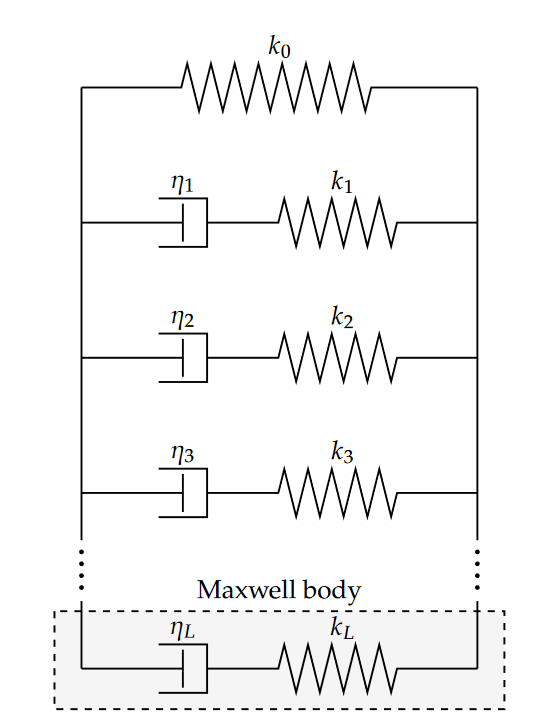
\includegraphics[width=7cm]{figures/gsls.png}
    \caption{Schematic diagram of a generalized standard linear solid (GSLS) composed of $L$ relaxation mechanisms (or Maxwell bodies), highlighted by the dashed square. $k_i$ ($i=1,\dots,L$) and $\eta_i$ ($i=1,\dots,L$) represent the elastic moduli and Newtonian viscosities, respectively, and are connected with the stress relaxation times $\tau^{\sigma l}$ and strain retardation times $\tau^{\varepsilon l}$ via $\tau^{\sigma l}=\frac{\eta_l}{k_l}$ and $\tau^{\varepsilon l}=\frac{\eta_l}{k_0}+\frac{\eta_l}{k_l}$ (after \cite{zener:48}; \cite{bohlen:02}).}
    \label{fig:gsls}
\end{figure}

With such a setup, new parameters are introduced:
\begin{itemize}
    \item $\tau^{\sigma l}$ and $\tau^{\varepsilon l}$: \textbf{stress-relaxation time} and \textbf{strain-retardation time}, respectively, of the $l$-th relaxation mechanism,
    \item $C^R$: \textbf{relaxed (or equilibrium) modulus}, i.e., $\lim_{t\to\infty} C(t)$ (where $C(t)$ represents the stress-impulse response function of the viscoelastic medium), corresponding to the low-frequency limit, i.e., $\omega = 0$.
\end{itemize}
According to \citet{Bai:16}, each relaxation process can be expressed in terms of the stress relaxation function $\Psi_{ijkl}(t)$ of the GSLS as\footnote{The differential calculus is firstly done in the Laplace domain and then back-transformed to the time domain.}
\begin{equation}
    \Psi_{ijkl}(t) = C_{ijkl}^R\,\left[1+\sum_{l=1}^{L} \left(\frac{\tau_{ij}^{\varepsilon l}}{\tau^{\sigma l}}-1\right) \exp\left(-\frac{t}{\tau^{\sigma l}}\right) \right] H(t)\;.
    \label{eq:psi}
\end{equation}
To simplify equation~\ref{eq:psi}, \citet{blanch:95} introduced the $\tau$-method, which demonstrates that the magnitude of attenuation in anisotropic media is directly quantified by the dimensionless matrix $\tau_{ij}$, which generally describes the \textbf{attenuation parameters} (directional variation of attenuation):
\begin{equation}
    \tau_{ij} = \frac{\tau_{ij}^{\varepsilon l}}{\tau^{\sigma l}}-1\;.
    \label{eq:taumethod}
\end{equation}
While $\tau_{ij}$ simply vanishes in the elastic case, as $\tau^{\sigma l} = \tau^{\varepsilon l}$, it should remain constant for all $L$ relaxation mechanisms in the viscoelastic case. In the previous studies, the attenuation was considered to be isotropic. We now included attenuation anisotropy as well.%This means that the number of independent parameters (i.e. $\tau^{\sigma l}$ and $\tau_{ij}$) for each element of $\Psi_{ijkl}$ reduces from 2$L$ to $L$+1 in the elastic case, while for the viscoelastic VTI case it is equal to $L$+4, i.e., $L$ for $\tau^{\sigma l}$ and 4 for $\tau_{ij}$. 

Considering the $\tau$-method, the explicit form of equation~\ref{eq:psi} is given by
\begin{equation}
    \Psi_{ijkl}(t) = C_{ijkl}^R\,\left[1+\sum_{l=1}^{L}\tau_{ij}\,\exp\left(-\frac{t}{\tau^{\sigma l}}\right) \right] H(t)\;.
    \label{eq:psi_2.0}
\end{equation}
Note that this relaxation function differs from the definition given in \citet{Bai:16}. In the special case of isotropy, $\Psi(t)$ reads  
\begin{subequations}
    \begin{align}
    \Psi_P(t) &= \pi\,\left[1+\sum_{l=1}^{L}\tau_P\,\exp\left(-\frac{t}{\tau^{\sigma l}}\right)\right]H(t)\;\\
    \Psi_S(t) &= \mu\,\left[1+\sum_{l=1}^{L}\tau_S\,\exp\left(-\frac{t}{\tau^{\sigma l}}\right)\right]H(t)\;.
    \end{align}
\end{subequations}

\citet{Bai:16} relate the relaxed modulus $C_{ijkl}^R$, corresponding to the model velocities, to the $C_{ijkl}$ modulus defined at the reference frequency $\omega_0 = 2\,\pi f_0$:
\begin{equation}
    C_{ijkl}^R = C_{ijkl}\bigg|_{\omega_0}\,\left(1+\sum_{l=1}^{L}\tau_{ij}\,\frac{(\omega_0\,\tau^{\sigma l})^2}{1+(\omega_0\,\tau^{\sigma l})^2} \right)^{-1}\;.
    \label{eq:relaxedmodulus_Bai}
\end{equation}
which, in the isotropic case, becomes
\begin{subequations}
\allowdisplaybreaks
\begin{align}
    \pi &= V_P^2\bigg|_{\omega_0}\;\rho\,\left(1+\sum_{l=1}^{L}\tau_P\,\frac{(\omega_0\,\tau^{\sigma l})^2}{1+(\omega_0\,\tau^{\sigma l})^2}\right)^{-1}\,,\\
    \mu &= V_S^2\bigg|_{\omega_0}\;\rho\,\left(1+\sum_{l=1}^{L}\tau_S\,\frac{(\omega_0\,\tau^{\sigma l})^2}{1+(\omega_0\,\tau^{\sigma l})^2}\right)^{-1}\;.
\end{align}
\end{subequations}

Following \citet{Zhu:06} and equation~\ref{eq:relaxedmodulus_Bai}, the mathematical matrix representation of $Q$ is given by 
\enlargethispage{\baselineskip}
\begin{equation}
    Q_{ij}^{-1}(\omega,\tau^{\sigma l},\tau_{ij}) = \frac{\sum_{l=1}^{L}\tau_{ij}\,\frac{\omega\tau^{\sigma l}}{1+(\omega\tau^{\sigma l})^2}}{1+\sum_{l=1}^{L}\tau_{ij}\,\frac{(\omega\tau^{\sigma l})^2}{1+(\omega\tau^{\sigma l})^2}}\;,
    \label{eq:Qinverse}
\end{equation}
with the substitutions $\tau = \tau_P$ and $\tau = \tau_S$, in the special case of isotropy, defining the level of attenuation for P- and S-waves, respectively. In general, the width of the frequency range in which a nearly constant $Q_{ij}$-spectrum can be simulated directly depends on the number of relaxation mechanisms (\cite{Bai:16}; \cite{Komatitisch:99}). When a GSLS consists of only one relaxation mechanism, i.e., $L=1$, a good estimate for $\tau$ is $\tau = \frac{2}{Q}$ (\cite{bohlen:02}).

At $t=0$, $\Psi_{ijkl}$ yields the \textbf{unrelaxed (or instantaneous) modulus} $C^U$, i.e., $\lim_{t\to0} C(t)$, which corresponds to the high-frequency limit, i.e., $\omega = \infty$.
\begin{equation}
    C_{ijkl}^U \equiv \Psi_{ijkl}\bigg|_{t=0} = C_{ijkl}^R\,(1+L\,\tau_{ij})\;,
\end{equation}
which, in the special case of isotropy, becomes
\begin{equation}
\allowdisplaybreaks
    \pi^U = \pi\,(1+L\,\tau_P)\quad\textrm{and}\quad\mu^U = \mu\,(1+L\,\tau_S)\;.
\end{equation}
By substituting $\Psi_{ijkl}(t)$ in the generalized stress-strain relation in viscoelastic media, and taking the time derivative on both sides, equation~\ref{eq:stress_strain_visco_2.0} becomes
\begin{equation}
\allowdisplaybreaks
    \begin{split}
    \dot{\sigma}_{ij} &= \dot{\Psi}_{ijkl}(t) \ast \dot{\varepsilon}_{kl} =\\ 
    &= C_{ijkl}^U\,\dot{\varepsilon}_{kl}-(C_{ijkl}^U-C_{ijkl}^R) \left[ \sum_{l=1}^{L}\frac{1}{\tau^{\sigma l}}\exp\left(-\frac{t}{\tau^{\sigma l}}\right) \right]H(t) \ast \dot{\varepsilon}_{kl}\;.
    \label{eq:stress_vti}
    \end{split}
\end{equation}
which, in isotropic anelastic media, is given by
\begin{equation}
    \sigma_{ij} = (\dot{\Psi}_P - 2\dot{\Psi}_S) \ast \theta\,\delta_{ij} + 2\,\dot{\Psi}_S \ast \varepsilon_{ij}\,.
    \label{eq:stress_iso_visco}
\end{equation}
In order to replace the convolution terms, \citet{Carcione:88} and \citet{robertsson:94} suggested that \textbf{memory variables} $r_{ij}^l$ corresponding to the $ij$-th component for the $l$-th relaxation mechanism should be introduced in such a way that
\begin{equation}
\allowdisplaybreaks
    r_{ij}^l = -\frac{2}{L\,\tau^{\sigma l}}\,(C_{ijkl}^U-C_{ijkl}^R)\exp\left(-\frac{t}{\tau^{\sigma l}}\right)H(t) \ast \dot{\varepsilon}_{kl}\;,
    \label{eq:r}
\end{equation}
which becomes by differentiating with respect to time and rearranging
% \begin{equation}
% \allowdisplaybreaks
%     \dot{r}_{ij}^l = \left[ -\frac{1}{\tau^{\sigma l}}(C_{ijkl}^U-C_{ijkl}^R)\,\exp\left(-\frac{t}{\tau^{\sigma l}}\right)\right] \left(-\frac{1}{\tau^{\sigma l}}\, H(t) + \delta(t)\right) \ast \dot{\varepsilon}_{kl}\;.
% \end{equation}
\begin{equation}
\allowdisplaybreaks
    \begin{split}
    \dot{r}_{ij}^l = &-\frac{2}{L\,\tau^{\sigma l}}\, \left[ -\frac{1}{\tau^{\sigma l}}(C_{ijkl}^U-C_{ijkl}^R)\,\exp\left(-\frac{t}{\tau^{\sigma l}}\right)H(t) \ast \dot{\varepsilon}_{kl} \right] - \\
    &- \frac{2}{L\,\tau^{\sigma l}}\,(C_{ijkl}^U-C_{ijkl}^R)\exp\left(-\frac{t}{\tau^{\sigma l}}\right)\,\delta(t) \ast \dot{\varepsilon}_{kl}\;.
    \end{split}
    \label{eq:r_dot}
\end{equation}
Introducing the expression of $r_{ij}^l$ at $t=0$ in equation~\ref{eq:r_dot}, I get
\begin{equation}
\allowdisplaybreaks
    \dot{r}_{ij}^l = - \frac{2}{L\,\tau^{\sigma l}}\,\left[ \frac{1}{2}\,(C_{ijkl}^U-C_{ijkl}^R)\left(\frac{\partial v_k}{\partial x_l}+\frac{\partial v_l}{\partial x_k}\right)+r_{ij}^l \right]\;.
    \label{eq:final_r_dot}
\end{equation}
Thus, equation \ref{eq:stress_vti} becomes
\begin{equation}
    \dot{\sigma}_{ij} = C_{ijkl}^U\,\left(\frac{\partial v_k}{\partial x_l}+\frac{\partial v_l}{\partial x_k}\right)+\sum_{l=1}^{L}r_{ij}^l\;.
    \label{eq:stress_vti_final}
\end{equation}
which, in the special case of isotropy, reads
\begin{equation}
    \dot \sigma_{ij} = \left[\pi\,(1+L\,\tau_{\varepsilon l}^P)-2\mu\,(1+L\,\tau_{\varepsilon l}^S)\right]\frac{\partial v_k}{\partial x_k}\,\delta_{ij} + \mu\,(1+L\,\tau_{\varepsilon l}^S)\left(\frac{\partial v_i}{\partial x_j}+\frac{\partial v_j}{\partial x_i}\right) + \sum_{l=1}^{L}r_{ij}^l\;.
\end{equation}

\subsection{Equations of motion for an anisotropic medium}
\label{ch:anisotropy}

\subsubsection{Seismic anisotropy and elasticity tensor}
As opposed to isotropy, which means homogeneity in all directions, anisotropy is the property of directional dependency. In seismics, anisotropy describes the directional or angle dependence of the velocity of seismic waves in a medium within the Earth, which can help to characterize preferred orientation and in-situ stress conditions. If the rock properties are aligned over a greater volume extending several wavelengths, they can create certain symmetries of seismic anisotropy (\cite{Thomsen:86}). Hexagonal (or cylindrical) symmetry is of particular interest in seismics, as it is relatively simple but can still approximate many actual situations in the Earth, for instance where sedimentary layers are neatly ordered. The most typical anisotropic medium that exhibits hexagonal symmetry is \textbf{transversely isotropic}, which means that the velocity normal to the bedding is slower than the one along it. Commonly investigated symmetries are \textbf{vertical-transverse isotropy} (VTI), with a vertical symmetry axis and infinite number of horizontal planes with isotropic behavior, and \textbf{tilted-transverse isotropy} (TTI), with a rotated symmetry axis, and thus properties changing with azimuth (\cite{Tsvankin:12}) (see Fig.~\ref{fig:tti}). \citet{Bai:16} developed a detailed numerical demonstration and analysis of vertical-transverse isotropic attenuation by 2D time-domain finite-difference modeling, while \citet{Oh:20} developed a similar tilted-transverse version. 
\begin{figure}[h!]
    \centering
    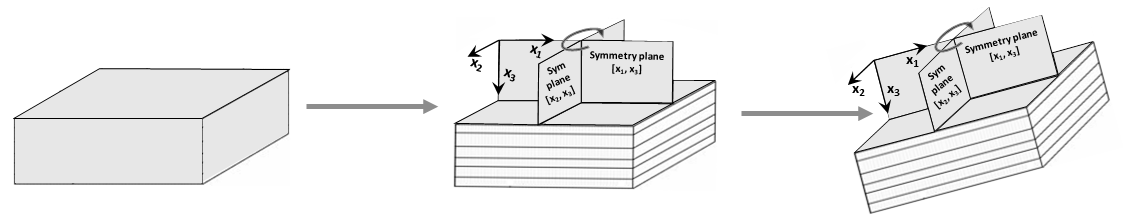
\includegraphics[width=0.9\textwidth]{figures/tti.png}
    \caption{From left to right: isotropic, VTI, and TTI media in a 3D Cartesian coordinate system with $(x_1,x_2,x_3) = (x,y,z)$ (modified after \cite{TGSwebsite}).}
    \label{fig:tti}
\end{figure}

The structure of the \textbf{stiffness tensor} $\mathbf{C_{ijkl}}$, previously introduced in subchapter~\ref{ch:eq_motion_elastic}, is the factor that determines the velocity and polarization of seismic waves for any propagation direction (\cite{Tsvankin:12}), thus uniquely describing the above-mentioned symmetries and their elastic moduli. In 3D, the fourth-order tensor had 36 independent components:
\begin{equation}
    \mathbf{C} = 
    \begin{pmatrix}
    c_{11} & c_{12} & c_{13} & c_{14} & c_{15} & c_{16} \\
    c_{12} & c_{22} & c_{23} & c_{24} & c_{25} & c_{26} \\
    c_{13} & c_{23} & c_{33} & c_{34} & c_{35} & c_{36} \\
    c_{14} & c_{24} & c_{34} & c_{34} & c_{45} & c_{46} \\
    c_{15} & c_{25} & c_{35} & c_{45} & c_{55} & c_{56} \\
    c_{16} & c_{26} & c_{36} & c_{46} & c_{56} & c_{66} 
    \end{pmatrix}\;,
    \label{eq:voigt_C}
\end{equation}
which is expressed in the Voigt notation (\cite{Voigt:10}).

For a polarization direction of the P-SV waves in 2D only, namely in the $x_1x_2$-plane, with the axes of the Cartesian coordinate system defined as $x_1$ for horizontal axis and $x_2$ for the vertical (depth) axis, the stiffness matrix becomes a $3 \times 3$ matrix with elements defining the $x_1x_1$-, $x_2x_2$-, and $x_1x_2$-directions. The stiffness tensor is then reduced to a combination of the Lam\'e parameters
\begin{equation}
    \mathbf{C} =
    \begin{pmatrix}
    c_{11} & c_{13} & c_{15} \\
    c_{13} & c_{33} & c_{35} \\
    c_{15} & c_{53} & c_{55} \\
    \end{pmatrix}\;.
    \label{eq:c_3x3}
\end{equation}
In the case of isotropic media, where the elastic behavior is independent of direction, only four elastic constants are independent and they simply reduce to
\begin{subequations}
\allowdisplaybreaks
    \begin{align}
        c_{11} &= c_{33}=\lambda+2\mu = \pi\;,\\
        c_{13} &= \lambda\;,\\
        c_{55} &= \mu\;,
    \end{align}
    \label{eq:c_iso_ij}
\end{subequations}
which form the elements of the stiffness matrix in 2D isotropic media:
\begin{equation}
    \mathbf{C}^\mathbf{iso} =
    \begin{pmatrix}
    \pi & \lambda & 0 \\
    \lambda & \pi & 0 \\
    0 & 0 & \mu \\
    \end{pmatrix}\;.
    \label{eq:c_iso_3x3}
\end{equation}
The P- and S-wave velocities will read then as
\begin{subequations}
\allowdisplaybreaks
    \begin{align}
        v_{P,ver} &= \sqrt{\frac{\lambda+2\mu}{\rho}}\;,\\
        v_{SV,ver} &= \sqrt{\frac{\mu}{\rho}}\;.
    \end{align}
\end{subequations}
In the case of 2D VTI media, Eq.~\ref{eq:c_3x3} reads (\cite{Thomsen:86})
\begin{equation}
    \mathbf{C}^\mathbf{VTI} =
    \begin{pmatrix}
    c_{11} & c_{13} & 0 \\
    c_{13} & c_{33} & 0 \\
    0 & 0 & c_{55} \\
    \end{pmatrix}\;.
    \label{eq:c_vti_3x3}
\end{equation}
Under the assumption of weak anisotropy, i.e., less than 20\%, these independent elastic constants have been combined by \citet{Thomsen:86} into the so-called \textbf{Thomsen anisotropic parameters} $\varepsilon$ and $\delta$ (dimensionless), such that they can better describe the seismic wave propagation:
\begin{subequations}
\allowdisplaybreaks
\begin{align}
    \varepsilon &= \frac{c_{11}-c_{33}}{2c_{33}}\;,\\
    \delta &= \frac{(c_{13}+c_{55})^2-(c_{33}-c_{55})^2}{2c_{33}\,(c_{33}-c_{55})}\;.
\end{align}
\end{subequations}
The vertical P- and S-wave velocities can also be expressed in terms of these elastic constants:
\begin{equation}
    v_{P,ver} \equiv \sqrt{\frac{c_{33}}{\rho}} \quad \textrm{and} \quad v_{SV,ver} \equiv \sqrt{\frac{c_{55}}{\rho}}\;.
    \label{eq:ver_vel}
\end{equation}

The angle-dependency of phase velocities, with the angle $\theta$ made by the symmetry axis of the VTI medium with the normal of the wavefront, is then given by the following approximate expressions:
\begin{subequations}
\allowdisplaybreaks
\begin{align}
    v_P(\theta) &\approx v_{P,ver}\,(1+\delta\,\sin^2\theta\cos^2\theta+\varepsilon\,\sin^4\theta)\;,\\
    v_{SV}(\theta) &\approx v_{SV,ver}\,\left(1+\frac{v_{P,ver}^2}{v_{SV,ver}^2}\,(\varepsilon-\delta)\sin^2\theta\,\cos^2\theta\right)\;,
    \label{eq:vel_angle}
\end{align}
\end{subequations}
with the maximal P-wave velocity given for a horizontal direction of wave propagation, while the maximal S-wave is reached at $45^{\circ}$:
\begin{subequations}
    \begin{align}
    v_{P,hor} &\equiv v_{P,ver}\,(1+\varepsilon)\;,\\
    v_{S,45^{\circ}} &\equiv \frac{v_{P,hor}^2\,(\varepsilon-\delta)}{4\,v_{SV,ver}}+v_{SV,ver}\;.
    \end{align}
    \label{eq:v_aniso}
\end{subequations}
In the case of $C_{ijkl}$ set along the symmetry axis, i.e., $\theta=0^{\circ}$, the elements of the stiffness matrix $\mathbf{C}^\mathbf{VTI}$ in Eq.~\ref{eq:c_vti_3x3} can be expressed as
\begin{equation}
    \renewcommand{\arraystretch}{2}
    \begin{pmatrix}
    c_{11} \\
    c_{33} \\
    c_{13} \\
    c_{55}
    \end{pmatrix} = 
    \begin{pmatrix}
    \rho\,v_{P,ver}^2\,(1+2\,\varepsilon) \\
    \rho\,v_{P,ver}^2 \\
    \rho\,\left(\sqrt{\left(v_{P,ver}^2-v_{SV,ver}^2\right)\left[v_{P,ver}^2\,\left(1+2\,\delta\right)-v_{SV,ver}^2\right]}-v_{SV,ver}^2\right) \\
    \rho\,v_{SV}^2 
    \end{pmatrix}\;.
    \label{eq:c_vti_thomsen}
\end{equation}
It can be observed that, while $\varepsilon$ quantifies the velocity difference for wave propagation along and perpendicular to the symmetry axis, $\delta$ controls the P-wave propagation for angles near the symmetry axis. 

In the case of TTI media, the stiffness matrix can be derived from the $\mathbf{C}^\mathbf{VTI}$ using the Bond transformation (\cite{Bond:43}; \cite{Carcione:07}) as suggested by \citet{Oh:20}: 
\begin{equation}
    \Tilde{\mathbf{C}}^\mathbf{TTI} = D(\theta_T)\,\mathbf{C}^{VTI}\,D^T(\theta_T)\;,
\end{equation}
with 
\begin{equation}
    D(\theta_T) = 
    \begin{pmatrix}
    \cos^{2}\theta_T & \sin^{2}\theta_T & 2\sin\theta_T\cos\theta_T \\
    \sin^{2}\theta_T & \cos^{2}\theta_T & -2\sin\theta_T\cos\theta_T \\
    -\sin\theta_T\cos\theta_T & \sin\theta_T\cos\theta_T & -\sin^{2}\theta_T \\
    \end{pmatrix}\,.
    \label{eq:d_vti}
\end{equation}
The matrix $\textit{D}$, rotated about the vertical axis in a counter-clockwise direction, represents a simple coordinate-rotation matrix, and the parameter $\theta_T$ denotes the tilt angle of the symmetry axis measured from the vertical. With its general expression given by
\begin{equation}
    \Tilde{\mathbf{C}}^\mathbf{TTI} = 
    \begin{pmatrix}
    \Tilde{c}_{11} & \Tilde{c}_{13} & \Tilde{c}_{15} \\
    \Tilde{c}_{13} & \Tilde{c}_{33} & \Tilde{c}_{35} \\
    \Tilde{c}_{15} & \Tilde{c}_{35} & \Tilde{c}_{55} \\
    \end{pmatrix}\,,
    \label{eq:c_tti_3x3}
\end{equation}
the $\tilde{c}_{ij}$ elements can be explicitly defined as
\begin{equation}
    \begin{pmatrix}
    \Tilde{c}_{11} \\
    \Tilde{c}_{33} \\
    \Tilde{c}_{13} \\
    \Tilde{c}_{55} \\
    \Tilde{c}_{15} \\
    \Tilde{c}_{35} \\
    \end{pmatrix} = 
    \begin{pmatrix}
    c_{11}\cos^{4}\theta_T+c_{33}\sin^{4}\theta_T+2\,(c_{13}+4\,c_{55})\,\sin^{2}\theta_T\cos^{2}\theta_T \\
    c_{11}\sin^{4}\theta_T+c_{33}\cos^{4}\theta_T+2\,(c_{13}+4\,c_{55})\,\sin^{2}\theta_T\cos^{2}\theta_T \\
    (c_{11}+c_{33}-4\,c_{55})\,\sin^{2}\theta_T\cos^{2}\theta_T+c_{13}\,(\sin^{4}\theta_T+\cos^{4}\theta_T) \\
    (c_{11}+c_{33}-2\,c_{13})\,\sin^{2}\theta_T\cos^{2}\theta_T+c_{55}\,(\cos^{2}\theta_T-\sin^{2}\theta_T)^2 \\
    (c_{13}-c_{11}+2\,c_{55})\,\cos^{3}\theta_T\sin\theta_T-(c_{13}-c_{33}+2\,c_{55})\,\cos\theta_T\sin^{3}\theta_T \\
    (c_{13}-c_{11}+2\,c_{55})\,\sin^{3}\theta_T\cos\theta_T-(c_{13}-c_{33}+2\,c_{55})\,\sin\theta_T\cos^{3}\theta_T \\ 
    \end{pmatrix}\;.
    \label{eq:c_tti_3x3_explicit}
\end{equation}

\subsubsection{Wave equations}
In this section, the velocity-stress formulation of the system of first-order differential equations that are the basis for the 2D FD anisotropic implementation is given. The wave equation for the 2D viscoelastic TTI media has been implemented recently into SOFI2D in order to verify the consistency of our extended wave equation formulation for anisotropic media with our previous formulation for isotropic media. 

For elastic media:
\begin{itemize}
    \item isotropic wave equations
        \begin{subequations}
        \allowdisplaybreaks
        \begin{align}
            % \rho\dot{v_x} &= \frac{\partial \sigma_{xx}}{\partial x} + \frac{\partial \sigma_{xz}}{\partial z}\;,\\
            % \rho\dot{v_z} &= \frac{\partial \sigma_{xz}}{\partial x} + \frac{\partial \sigma_{zz}}{\partial z}\;,\\
            \dot{\sigma}_{xx} &= \pi\,\frac{\partial v_x}{\partial x} + \lambda\,\frac{\partial v_z}{\partial z}\;,\\
            \dot{\sigma}_{zz} &= \lambda\,\frac{\partial v_x}{\partial x} + \pi\,\frac{\partial v_z}{\partial z}\;,\\
            \dot{\sigma}_{xz} &= \mu\,\left(\frac{\partial v_x}{\partial z} + \frac{\partial v_z}{\partial x}\right)\;.
            \label{eq:iso_elastic} 
        \end{align}
        \end{subequations}
    \item VTI wave equations
        \begin{subequations}
            \allowdisplaybreaks
            \begin{align}
            % \rho\dot{v_x} &= \frac{\partial \sigma_{xx}}{\partial x} + \frac{\partial \sigma_{xz}}{\partial z}\;,\\
            % \rho\dot{v_z} &= \frac{\partial \sigma_{xz}}{\partial x} + \frac{\partial \sigma_{zz}}{\partial z}\;,\\
            \dot{\sigma}_{xx} &= c_{11}\,\frac{\partial v_x}{\partial x} + c_{13}\,\frac{\partial v_z}{\partial z}\;,\\
            \dot{\sigma}_{zz} &= c_{13}\,\frac{\partial v_x}{\partial x} + c_{33}\,\frac{\partial v_z}{\partial z}\;,\\
            \dot{\sigma}_{xz} &= c_{55}\left(\frac{\partial v_x}{\partial z} + \frac{\partial v_z}{\partial x}\right)\;.
            \label{eq:vti_elastic} 
            \end{align}
        \end{subequations}
    \item TTI wave equations
        \begin{subequations}
            \allowdisplaybreaks
            \begin{align}
            % \rho\dot{v_x} &= \frac{\partial \sigma_{xx}}{\partial x} + \frac{\partial \sigma_{xz}}{\partial z}\;,\\
            % \rho\dot{v_z} &= \frac{\partial \sigma_{xz}}{\partial x} + \frac{\partial \sigma_{zz}}{\partial z}\;,\\
            \dot{\sigma}_{xx} &= \tilde{c}_{11}\,\frac{\partial v_x}{\partial x} + \tilde{c}_{13}\,\frac{\partial v_z}{\partial z}\ + \tilde{c}_{15}\,\left(\frac{\partial v_x}{\partial z} + \frac{\partial v_z}{\partial x}\right)\;,\\
            \dot{\sigma}_{zz} &= \tilde{c}_{13}\,\frac{\partial v_x}{\partial x} + \tilde{c}_{33}\,\frac{\partial v_z}{\partial z}\ + \tilde{c}_{35}\,\left(\frac{\partial v_x}{\partial z} + \frac{\partial v_z}{\partial x}\right)\;,\\
            \dot{\sigma}_{xz} &= \tilde{c}_{15}\,\frac{\partial v_x}{\partial x} + \tilde{c}_{35}\,\frac{\partial v_z}{\partial z}\ + \tilde{c}_{55}\,\left(\frac{\partial v_x}{\partial z} + \frac{\partial v_z}{\partial x}\right)\;.
            \label{eq:tti_elastic} 
            \end{align}
        \end{subequations}
\end{itemize}

The model parameters in the implementation of viscoelastic modeling are represented by the velocities and attenuation at $\omega_0$ and the relaxation frequencies $\tau^{\sigma l}$:
\begin{itemize}
    \item isotropic wave equations
        \begin{subequations}
        \allowdisplaybreaks
        \begin{align}
            \dot{\sigma}_{xx} &= \pi\,(1+L\,\tau^P)\,\left(\frac{\partial v_x}{\partial x} + \frac{\partial v_z}{\partial z} \right) - 2\,\mu\,(1+L\,\tau^S)\,\frac{\partial v_z}{\partial z} + \sum_{l=1}^{L}r_{xx}^l\;,\\   
            \dot{\sigma}_{zz} &= \pi\,(1+L\,\tau^P)\,\left(\frac{\partial v_x}{\partial x} + \frac{\partial v_z}{\partial z} \right) - 2\,\mu\,(1+L\,\tau^S)\,\frac{\partial v_x}{\partial x} + \sum_{l=1}^{L}r_{zz}^l\;,\\   
            \dot{\sigma}_{xz} &= \mu\,(1+L\,\tau^S)\,(\frac{\partial v_x}{\partial z}+\frac{\partial v_z}{\partial x})+\sum_{l=1}^{L}r_{xz}^l\;,\\    
            \dot{r}_{xx}^l &= -\frac{1}{\tau^{\sigma l}}\, \left[\pi\,\tau^P\,\left(\frac{\partial v_x}{\partial x} + \frac{\partial v_z}{\partial z} \right) - 2\,\mu\,\tau^S\,\frac{\partial v_z}{\partial z} + r_{xx}^l \right]\;,\\ 
            \dot{r}_{zz}^l &= -\frac{1}{\tau^{\sigma l}}\, \left[\pi\,\tau^P\,\left(\frac{\partial v_x}{\partial x} + \frac{\partial v_z}{\partial z} \right) - 2\,\mu\,\tau^S\,\frac{\partial v_x}{\partial x} + r_{zz}^l \right]\;,\\ 
            \dot{r}_{xz}^l &= -\frac{1}{\tau^{\sigma l}}\, \left[\mu\,\tau^S\,\left(\frac{\partial v_x}{\partial x} + \frac{\partial v_z}{\partial z} \right) + r_{xz}^l \right]\;.
        \end{align}
        \end{subequations}
    \item VTI media
        \begin{subequations}
        \allowdisplaybreaks
        \begin{align}
            \dot{\sigma}_{xx} &= c_{11}^U\,\frac{\partial v_x}{\partial x}+c_{13}^U\,\frac{\partial v_z}{\partial z}+\sum_{l=1}^{L}r_{xx}^l\;,\\   
            \dot{\sigma}_{zz} &= c_{13}^U\,\frac{\partial v_x}{\partial x}+c_{33}^U\,\frac{\partial v_z}{\partial z}+\sum_{l=1}^{L}r_{zz}^l\;,\\   
            \dot{\sigma}_{xz} &= c_{55}^U\,\left(\frac{\partial v_x}{\partial z}+\frac{\partial v_z}{\partial x}\right)+\sum_{l=1}^{L}r_{xz}^l\;,\\     
            \dot{r}_{xx}^l &= -\frac{1}{\tau^{\sigma l}}\,\left(c_{11}^R\,\tau_{11}\,\frac{\partial v_x}{\partial x}+c_{13}^R\,\tau_{13}\,\frac{\partial v_z}{\partial z}+r_{xx}^l\right)\;,\\
            \dot{r}_{zz}^l &= -\frac{1}{\tau^{\sigma l}}\, \left(c_{13}^R\,\tau_{13}\,\frac{\partial v_x}{\partial x}+c_{33}^R\,\tau_{33}\,\frac{\partial v_z}{\partial z}+r_{zz}^l \right)\,,\\
            \dot{r}_{xz}^l &= -\frac{1}{\tau^{\sigma l}}\, \left[c_{55}^R\,\tau_{55}\,\left(\frac{\partial v_x}{\partial z}+\frac{\partial v_z}{\partial x}\right)+r_{xz}^l \right]\;.
            \label{eq:wave_eq_vti}
        \end{align}
        \end{subequations}
    \item TTI media
        \begin{subequations}
        \allowdisplaybreaks
        \begin{align}
            \dot{\sigma}_{xx} &= \Tilde{c}_{11}^U\,\frac{\partial v_x}{\partial x}+\Tilde{c}_{13}^U\,\frac{\partial v_z}{\partial z}+\Tilde{c}_{15}\,\left(\frac{\partial v_x}{\partial z}+\frac{\partial v_z}{\partial x}\right)+\sum_{l=1}^{L}r_{xx}^l\;,\\   
            \dot{\sigma}_{zz} &= 
            \Tilde{c}_{13}^U\,\frac{\partial v_x}{\partial x}+\Tilde{c}_{33}^U\,\frac{\partial v_z}{\partial z}+\Tilde{c}_{35}\,\left(\frac{\partial v_x}{\partial z}+\frac{\partial v_z}{\partial x}\right)+\sum_{l=1}^{L}r_{zz}^l\;,\\
            \dot{\sigma}_{xz} &= \Tilde{c}_{15}^U\,\frac{\partial v_x}{\partial x}+\Tilde{c}_{35}^U\,\frac{\partial v_z}{\partial z}+\Tilde{c}_{55}\,\left(\frac{\partial v_x}{\partial z}+\frac{\partial v_z}{\partial x}\right)+\sum_{l=1}^{L}r_{xz}^l\;,\\
            -\tau_{\sigma l}\,\dot{r}_{xx}^l &=  \Tilde{c}_{11}^R\,\tau_{11}\,\frac{\partial v_x}{\partial x}+\Tilde{c}_{13}^R\,\tau_{13}\,\frac{\partial v_z}{\partial z}+\Tilde{c}_{15}^R\,\tau_{13}\,\left(\frac{\partial v_x}{\partial z}+\frac{\partial v_z}{\partial x}\right)+r_{xx}^l\;,\\
            -\tau_{\sigma l}\,\dot{r}_{zz}^l &=  \Tilde{c}_{33}^R\,\tau_{33}\,\frac{\partial v_z}{\partial z}+\Tilde{c}_{13}^R\,\tau_{13}\,\frac{\partial v_x}{\partial x}+\Tilde{c}_{35}^R\,\tau_{35}\,\left(\frac{\partial v_x}{\partial z}+\frac{\partial v_z}{\partial x}\right)+r_{zz}^l\;,\\
            -\tau_{\sigma l}\,\dot{r}_{xz}^l &=  \Tilde{c}_{55}^R\,\tau_{55}\,\left(\frac{\partial v_z}{\partial x}+\frac{\partial v_x}{\partial z}\right)+\Tilde{c}_{15}^R\,\tau_{15}\,\frac{\partial v_x}{\partial x}+\Tilde{c}_{35}^R\,\tau_{35}\,\frac{\partial v_z}{\partial z}+r_{xz}^l\;.
            \label{eq:wave_eq_tti}
        \end{align}
        \end{subequations}
\end{itemize}

\subsubsection{Numerical results}
In order to emphasize the pronounced effects of anisotropy on the wavefield, we show the directional variation of P- and S-waves in a highly anisotropic VTI medium (Fig.~\ref{fig:snapshots}). The P-wave velocity increases significantly towards the horizontal direction ($\theta = \ang{90}$). The angular variation of S-wave depends upon polarity. Horizontally polarized S-waves (SH) are fastest in the horizontal direction, whereas vertically polarized S-waves (SV) have a maximum velocity around $\theta = \ang{45}$.

We also compare numerical results for the elastic and viscoelastic
case to highlight the effects of attenuation. Whereas attenuation mainly leads to a frequency dependent decay of amplitudes with distance, anisotropy affects both travel times and amplitudes considerably. Note for instance the strong deformation of both the P- and SV-wave wavefronts in the VTI case according to the directional variation of phase velocities depicted in Fig.~\ref{fig:snapshots}. Furthermore, in the VTI medium the SV-wave develops significant amplitude anomalies along the diagonal direction ($\theta = \ang{45}$), known as cusps. The counter-clockwise rotation of the symmetry axis in the TTI case by $\theta = \ang{30}$ is clearly visible and has a strong impact on the radiation pattern of the wavefield for both P- and SV-waves.

\begin{figure}[h!]
    \centering
    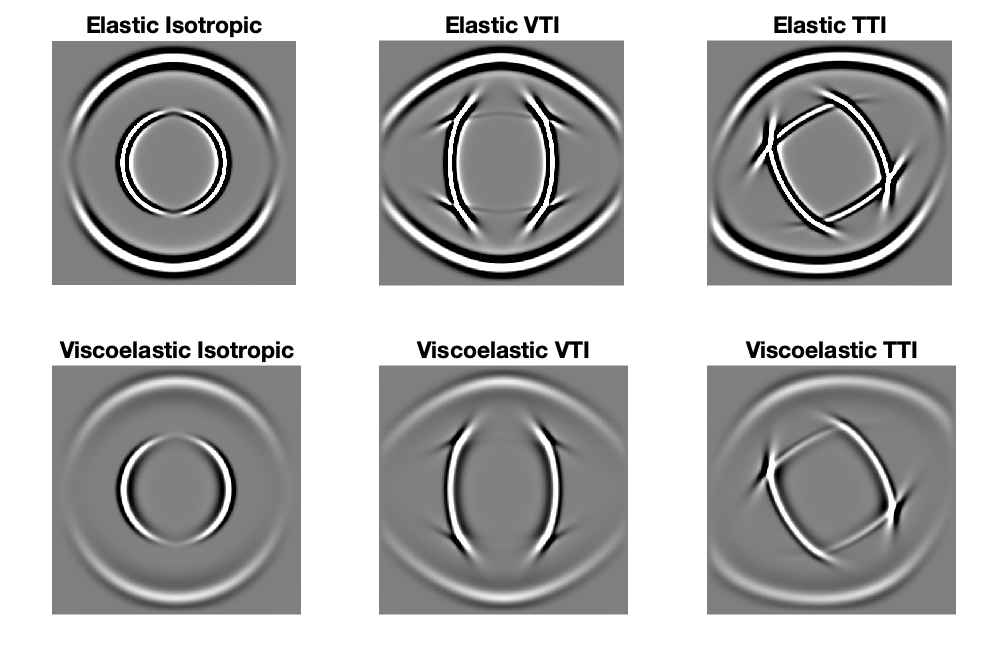
\includegraphics[width=0.9\textwidth]{figures/modeling}
    \caption{Snapshots of vertical component of particle velocity excited by a vertical point force. The snapshots show P- and SV-waves and the effects of attenuation and VTI and TTI anisotropy. The homogeneous anisotropic VTI model is that of Greenhorn shale. In the TTI model, the symmetry axis has been rotated counter-clockwise $\theta = \ang{30}$. Attenuation is assumed to be isotropic and described by $\sigma_P=\sigma_S=\SI{0.25}{}$, $L=1$.}
    \label{fig:snapshots}
\end{figure}

\subsection{Solution of the wave equation by finite differences}
\label{elastic_FD_Code}
Solving the above-mentioned wave equations analytically is only possible for very simple models. In more realistic cases, wave propagation can only be estimated using numerical approaches. One of them is the \textbf{finite-differences (FD) method}, in which spatial and temporal derivatives in the wave equations are approximated by FD operators, making it numerical efficient and relatively straightforward to implement. This approximation requires the discretization of the wave equation in both space and time using a Cartesian coordinate system of equidistant grid spacing. Thus, the continuous space coordinates $x$ and $z$ and the time vector $t$ are replaced by their discrete form in a way that $x = i\,\Delta h$, $z = j\,\Delta h$, and $t = n\,\Delta t$, with $i,j$ representing the position of a specific grid point and $n$ referring to a specific \textbf{time step}; $\Delta h$ denotes the spatial distance between two adjacent grid points (i.e., \textbf{grid spacing}) and $\Delta t$ the difference between two successive time steps (i.e., time sampling interval). Therefore, every grid point is located in the interval  $i \in N | [1,NX]$, $j \in N | [1,NY]$ and $n \in N | [1,NT]$, where $NX$, $NY$ and $NT$ are the number of discrete spatial grid points and time steps, respectively. 

Two types of operators can be distinguished, forward and backward operators $D^+,D^-$. The derivative of a function $y$ with respect to a variable $x$ can be approximated by the following operators:  
\begin{subequations}
    \begin{align}
        {D^+_x} y &= \frac{y{[i+1]} - {y[i]}}{\Delta h}\;,\\
        {D^-_x} y &= \frac{y{[i]}-y{[i-1]}}{\Delta h}\;.
    \end{align}
    \label{eq:3}
\end{subequations}

\subsubsection{Standard staggered grid}
\label{ssg}
The propagation of elastic waves in the stress-velocity formulation can be modeled on a standard staggered grid (SSG), which ensures stability and high accuracy (\cite{virieux:86}; \cite{levander:88}). On such a grid, different components of one physical parameter are defined at different staggered points. Fig.~\ref{fig:ssg} shows the locations of viscoelastic wavefield parameters and material parameters on the SSG. Fig.~\ref{fig:ssg} shows the locations of wavefield parameters: the two different components of the particle velocity $v_i$ are distributed over two different staggered locations, at half grid points; the stress components $\sigma_{ij}$ are distributed over two different locations: the diagonal stresses on full grid points, and the shear stresses on half grid points; the same holds for the memory variables.

The material parameters, namely $\rho$, $\mu$, $\tau$, and the $c_{ij}$ components need to be locally averaged, i.e., calculated from neighboring grid points. The averaging of material parameters is critical for the accuracy at strong discontinuities \cite{zahradnik:93,falk:98,moczo:02}. To obtain stable results, arithmetic averaging  must be used for the density $\rho$ and attenuation parameter $\tau^S$, and harmonic averaging is required for the shear modulus (\cite{fellinger:95,graves:96,falk:98,vossen:02,moczo:02}):
\begin{subequations}
\allowdisplaybreaks
    \begin{align}
        \rho_x[j,i+\frac{1}{2}] &= \frac{\rho[j,i]+\rho[j,i+1]}{2}\;,\\
        \rho_y[j+\frac{1}{2},i] &= \frac{\rho[j,i]+\rho[j+1,i]}{2}\;,\\
        \tau^S_{xy}[j+\frac{1}{2},i+\frac{1}{2}] &= \frac{\tau^S[j,i]+\tau^S[j,i+1]+\tau^S[j+1,i+1]+\tau^S[j+1,i]}{4}\;,\\
        \mu_{xy}[j+\frac{1}{2},i+\frac{1}{2}] &= \frac{4}{\mu^{-1}[j,i]+\mu^{-1}[j,i+1]+\mu^{-1}[j+1,i+1]+\mu^{-1}[j+1,i]}\;.
        \label{eq:stress_vti}
    \end{align}
\end{subequations}
This averaging procedure satisfies the condition of traction continuity across the interface between two media on standard staggered grids (\cite{moczo:02}). Harmonic averaging of the shear modulus $\mu$ yields higher accuracy than arithmetic averaging for modeling Scholte waves propagating along fluid-solid interfaces (\cite{falk:98}). What is more, our numerical tests show that arithmetic averaging of the shear modulus across free surfaces leads to instabilities; harmonic averaging produces stable simulations. 
\begin{figure}[ht!]
    \centering
    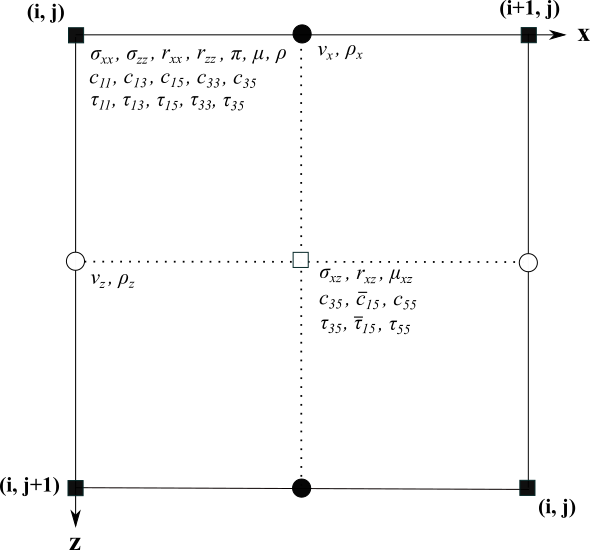
\includegraphics[width=10cm]{figures/ssg_final.png}
    \caption{Distribution of viscoelastic anisotropic wavefield- and material parameters on an elementary finite-difference cell in the standard staggered grid (modified after \cite{virieux:86}).
    At half grid point, i.e., $(i+\frac{1}{2},j+\frac{1}{2})$, $\bar{c}_{15}$ and $\bar{\tau}_{15}$ are harmonically- and arithmetically-averaged, respectively.}
    \label{fig:ssg}
\end{figure}

\subsubsection{Free surface and interfaces on a SSG}
% For the SSG the location of the free surface is defined by the plane going through the staggered position of the particle velocity $v_y$ and shear stress $\sigma_{xy}$ (Fig.~...). As a consequence the computation of the curl (S-wave component) and divergence (P-wave component) of the particle velocity wavefield is not accurate at the free surface because $v_x$ is located outside and $v_y$ inside the medium.
The determination of the actual location of an interface between two media on the SSG is not a trivial task. Only in the case that interfaces are aligned with the grid the interface location can be determined. On curved interfaces, however, the interface location cannot be determined exactly due to the staggered grid representation of the model. 

Varying topography in FD modeling can only be represented by staircases (Fig.~\ref{fig:ssg}). As the true topography can show strong variations in height, the topography on the SSG needs to be carefully handled. Following the distribution of physical parameters in an SSG cell, with the vertical component of the particle velocity calculated at half grid points, all vertical point sources and receivers must be located at half grid points, too, so that any numerical issues are avoided during modeling (Fig.~\ref{fig:ssg_topo}). 
\begin{figure}[ht!]
    \centering
    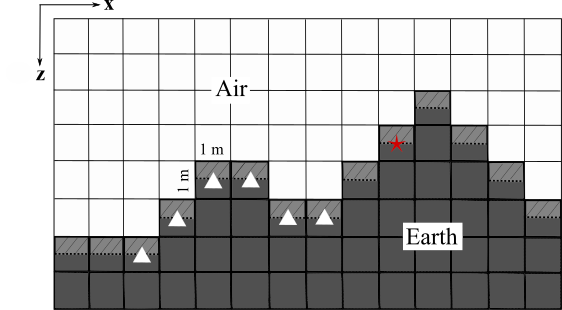
\includegraphics[width=9cm]{figures/topo.png}
    \caption{Topography on the standard staggered grid. Red star: source point; white triangles: receivers. Note the staircases that appear due to quantization of the elevation values.}
    \label{fig:ssg_topo}
\end{figure}

The interface between the elastic medium and air at the surface is very important when trying to model surface waves or multiple reflections in a marine environment. Since all stresses in the normal direction at this interface vanish in a way that $\sigma_{xy} = \sigma_{yy}=0.0$; this boundary condition is called (stress) {\textbf{free surface}}. Two types of implementations are common. \textcolor{red}{In the implicit definition of the free surface, a small layer with the acoustic parameters of air
($v_P=\SI{300}{m/s}$, $v_S=\SI{0}{m/s}$, $\rho=\SI{1.25}{kg/m^3}$) is placed on top of the model}. One advantage of the implicit definition of the free surface is the easy implementation of topography on the FD grid, however to get accurate results for surface waves or multiples, this approach requires a fine spatial sampling of the FD grid near the free surface. An explicit free surface can be implemented by using the mirroring technique by Levander, which leads to stable and accurate solutions for plain interfaces (\cite{levander:88}, \cite{robertsson:95}). If the planar free surface is located at grid point $j=h$, the stress at this point is set to zero and the stresses below the free surface are mirrored with an inverse sign:
\begin{equation}
\begin{split}
        \sigma_{yy}[h,i] &= 0\,,\\
        \sigma_{yy}[h-1,i] &= - \sigma_{yy}[h+1,i]\,,\\
        \sigma_{xy}[h-\frac{1}{2},i+\frac{1}{2}] &= - \sigma_{xy}[h+\frac{1}{2},i+\frac{1}{2}]\,,\\
        \sigma_{xy}[h-\frac{3}{2},i+\frac{1}{2}] &= - \sigma_{xy}[h+\frac{3}{2},i+\frac{1}{2}]\,.
\end{split}
\end{equation}

When updating the stress component $\sigma_{xx}=\Delta t\, \pi (v_{xx} + v_{yy}) -2 {\Delta t}\, \mu\, v_{yy}$ at the free surface only horizontal particle velocities should be used because vertical derivatives over the free surface lead to instabilities (\cite{levander:88}). 
The vertical derivative of $v_{yy}$ can be replaced by using the boundary condition at the free surface:
\begin{equation}
\begin{split}
    \sigma_{yy} &= {\Delta t}\, \pi\left(v_{xx} + v_{yy}\right)  - 2 {\Delta t}\, \mu\, v_{xx} = 0\;,\\
    v_{yy} &= - \frac{\pi-2\mu}{\pi} v_{xx}\;.
\end{split}
\end{equation}
Therefore equation ... can be written as
\begin{equation}
\sigma_{xx}={\Delta t}\left(4\mu -\frac{(2\mu)^2}{\pi} \right) v_{xx}\;.
\end{equation}

\subsubsection{Discretization of the wave equation}
\label{discretization}
The discretization of the linear stress-strain relationship at time step \textit{n} leads to the following system of equations:
\begin{equation}
\allowdisplaybreaks
    \begin{split}
        v_{xx}\,[j,i] & \approx \frac{v_x [j,i+\frac{1}{2}]-v_x[j,i-\frac{1}{2}]}{dh}\;,\\
        v_{yy}\,[j,i] & \approx \frac{v_y [j+\frac{1}{2},i]-v_y[j-\frac{1}{2},i]}{dh}\;,\\
        v_{yx}\,[j+\frac{1}{2},i+\frac{1}{2}] & \approx \frac{v_y [j+\frac{1}{2},i+1]-v_y [j+\frac{1}{2},i]}{\Delta h}\;,\\
        v_{xy}\,[j+\frac{1}{2},i+\frac{1}{2}] & \approx \frac{v_x  [j+1,i+\frac{1}{2}]-v_x [j,i+\frac{1}{2}]}{\Delta h}\;,\\
        \sigma_{xy}^{n}\,[j+\frac{1}{2},i+\frac{1}{2}] &= \sigma_{xy}^{n-1}\,[j+\frac{1}{2},i+\frac{1}{2}] + \Delta t \cdot \mu_{xy} \,[j+\frac{1}{2},i+\frac{1}{2}] \cdot\\
        & \cdot \biggl(v_{xy}\,[j+\frac{1}{2},i+\frac{1}{2}] + v_{yx} \,[j+\frac{1}{2},i+\frac{1}{2}]\biggr)\;,\\
        \sigma_{xx}^{n}\,[j,i] &= \sigma_{xx}^{n-1}\,[j,i] + \Delta t \cdot \pi [j,i] \cdot \biggl(v_{xx} [j,i] - v_{yy}\,[j,i] \biggr) - \\
        & -2 \cdot \Delta t \cdot \mu [j,i] \cdot v_{xx} [j,i]\;,\\
        \sigma_{yy}^{n}\,[j,i] &= \sigma_{yy}^{n-1}\,[j,i] + \Delta t \cdot \pi\,[j,i] \cdot \biggl(v_{xx}\,[j,i] - v_{yy}\,[j,i] \biggr) -\\
        & -2 \cdot dt \cdot \mu [j,i] \cdot v_{yy}\,[j,i]\;.
        \label{eq:discr_stress}
    \end{split}
\end{equation}
 
The discretization of the momentum equation leads to the following system of equations:
\begin{equation}
\allowdisplaybreaks
    \begin{split}
        vtt_x\,[j,i+\frac{1}{2}] &= \biggl(\sigma_{xx} [j,i+1] - \sigma_{xx}[j,i] + \sigma_{xy}[j+\frac{1}{2},i] - \sigma_{xy}[j-\frac{1}{2},i] \biggr)\;,\\
        vtt_y\,[j+\frac{1}{2},i] &= \biggl(\sigma_{xy}[j,i+\frac{1}{2}] - \sigma_{xy}[j,i-\frac{1}{2}] + \sigma_{yy} [j+1,i] - \sigma_{yy} [j,i] \biggr)\;,\\
        v_x^{n}\,[j,i+\frac{1}{2}] &= v_x^{n-1} [j,i+\frac{1}{2}] + \frac{\Delta t}{\Delta h}\cdot\rho_x  [j,i+\frac{1}{2}] \cdot vtt_x\,[j,i+\frac{1}{2}]\;,\\
        v_y^{n}\,[j+\frac{1}{2},i] &= v_y^{n-1} [j+\frac{1}{2},i] + \frac{\Delta t}{\Delta h} \cdot \rho_y [j+\frac{1}{2},i] \cdot vtt_y\,[j+\frac{1}{2},i]\;.\\
        \label{eq:discr_momentum}
    \end{split}
\end{equation}

\subsubsection{Accuracy of FD operators}
\label{accuracy}
The derivation of the FD operators in the last section was a simple replacement of the partial derivatives by finite differences. In the following more systematic approach, the first derivative of a variable $f$ at a grid point $i$ is estimated by a Taylor series expansion (\cite{jastram:92a}):
\begin{equation}
    \begin{split}
        (2k-1)\frac{\partial f}{\partial x}\biggr|_i &= \frac{1}{\Delta h}(f_{i+(k-1/2)}-f_{i-(k-1/2)}) + \\
        & +\frac{1}{\Delta h}\sum_{l=2}^N \frac{((k-\frac{1}{2}) (\Delta h)^{2l-1}}{(2l-1)!}\frac{\partial^{(2l-1)}f}{\partial
        x^{(2l-1)}}\biggr|_i+{\mathcal{O}}(\Delta h)^{2N}\;.
    \end{split}
\end{equation}

For an operator with length $2N$, $N$ equations are added with a weight $\beta_k$:
\begin{equation}
    \begin{split}
        \biggl[\sum_{k=1}^{N} \beta_k (2k-1)\biggr]\frac{\partial f}{\partial x}\biggr|_i &= \frac{1}{\Delta h} \sum_{k=1}^{N} \beta_k (f_{i+(k-1/2)}-f_{i-(k-1/2)}) +\\
        &+\frac{1}{\Delta h}\sum_{k=1}^{N} \sum_{l=2}^N \beta_k \frac{((k-\frac{1}{2})(\Delta h)^{2l-1}}{(2l-1)!}\frac{\partial^{(2l-1)}f}{\partial
        x^{(2l-1)}}\biggr|_i+{\mathcal{O}}(\Delta h)^{2N}\;.
    \end{split}
\end{equation}

The case $N=1$ leads to the FD operator derived in the last section, which has a length of $2N=2$. The Taylor series is truncated after the first term (${\mathcal{O}}(\Delta h)^{2}$). Therefore, this operator is called {\textbf{2nd order FD operator}} which refers to the truncation error of the Taylor series and not to the order of the approximated derivative. To understand equation %\ER{op_acc:2} ...
better, we estimate a {\textbf{4th order FD operator}}. This operator has the length $2N=4$ or $N=2$. The sums in Eq. %\ER{op_acc:2} 
lead to:
\begin{equation}
    \begin{split}
        (\beta_1+3 \beta_2) \frac{\partial f}{\partial x}\biggr|_i &= \frac{1}{\Delta h}(\beta_1(f_{i+1/2}-f_{i-1/2})+\beta_2(f_{i+3/2}-f_{i-3/2})) +\\
        & +\frac{\Delta h^3}{\Delta h}\biggl[\beta_1\frac{1}{8 \cdot 3!}+\beta_2\frac{27}{8 \cdot 3!}\biggr]\frac{\partial^3 f}{\partial x^3}\biggr|_i\;.
    \end{split}
\end{equation}

The weights $\beta_k$ can be calculated by the following approach: 
The factor in front of the partial derivative on the LHS of Eq. %\ER{op_acc:3} 
should equal 1, therefore $\beta_1+3\beta_2=1$. The coefficients in front of $\frac{\partial^3 f}{\partial x^3}\biggr|_i$ on the RHS of Eq. %\ER{op_acc:3} 
should vanish: $\beta_1+27\beta_2=0$. The weights $\beta_k$ can be estimated by solving the matrix equation:
\begin{equation}
    \left(
    \begin{array}{ll}
    1 & 3 \\
    1 & 27 \\
    \end{array}
    \right)\cdot \hspace{0.2 cm}
    \left(
    \begin{array}{l}
    \beta_1 \\
    \beta_2 \\
    \end{array}
    \right)
    =
    \left(
    \begin{array}{l}
    1 \\
    0 \\
    \end{array}
    \right) \notag
\end{equation}

The resulting coefficients are $\beta_1=9/8$ and $\beta_2=-1/24$. Therefore, the 4th order backward- and forward operators are:
\begin{equation}
\begin{split}
    \frac{\partial f}{\partial x}\biggr|_{i+1/2} &= \frac{1}{\Delta h}[\beta_1 (f_{i+1}-f_i)+\beta_2 (f_{i+2}-f_{i-1})] \hspace{1 cm} \text{forward operator}\;,\\
    \frac{\partial f}{\partial x}\biggr|_{i-1/2} &= \frac{1}{\Delta h}[\beta_1 (f_{i}-f_{i-1})+\beta_2 (f_{i+1}-f_{i-2})] \hspace{1 cm} \text{backward operator}\;.
\end{split}
\end{equation}

The coefficients $\beta_i$ in the FD operator are called {\textbf{Taylor coefficients}}. The accuracy of higher order FD operators can be improved by seeking for FD coefficients $\beta_k$ that approximate the first derivative in a certain frequency range (\cite{holberg:87}). 
These numerically optimized coefficients are called {\textbf{Holberg coefficients}}.

\subsubsection{Adams-Bashforth fourth-order accurate time integrators}
\label{adams-bashforth}
To improve the precision of the temporal discretization the Adams-Bashforth fourth-order accurate time integrator can be used. 
The staggered Adams-Bashforth method (ABS) is a multi-step method that uses previously calculated wavefields to increase the accuracy order in time. In \citet{bohlen2015higher2} and \citet{bohlen2015higher} a detailed study of the performance of the ABS method in 1D and 3D is given. The analysis shows that the numerical dispersion is much lower than that of the widely used second-order leapfrog method. However numerical dissipation is introduced by the ABS method. In simulation experiments the convincing improvements of accuracy of the fourth-order ABS method is verified. For instance, in a realistic elastic 3D scenario the computing time reduces by a factor of approximately 2.2, whereas the memory requirements increase by approximately the same factor. The ABS method thus provides an alternative strategy to increase the time accuracy by investing computer memory instead of computing time.

In the following we provide an extract of \citet{bohlen2015higher2} to demonstrate the underlying theory. Additionally, seismograms of different temporal orders of accuracy and an analysis of the numerical simulation error are shown.

In SOFI2D, only a fourth-order accurate Adams-Bashforth time integrator is implemented, due to the superior performance over third-order.

\paragraph{Theory}
For the sake of simplicity, we illustrate the staggered ABS method using the 1D acoustic wave equation in velocity-stress formulation
\begin{subequations}
    \begin{align}
        \frac{\partial p(x,t)}{\partial t} &= - \pi (x)\,\frac{\partial v(x,t)}{\partial x}  \notag\;,\\
        \frac{\partial v(x,t)}{\partial t} &= -\rho^{-1}(x)\,\frac{\partial p(x,t)}{\partial x}\;.
        \label{waveequation}
    \end{align}
\end{subequations}
The wavefield variables are the pressure $p(x,t)$ and the particle velocity $v(x,t)$. The material is described by the P-wave modulus $\pi (x)$ and the mass density $\rho(x)$. For simplicity we omit the temporal ($t$) and spatial dependencies ($x$)  in the following.

Using the conventional second order staggered grid approximation to the first order time derivative we obtain
\begin{subequations}
    \begin{align}
    \frac{p |^{n+1/2}-p|^{n-1/2}}{\Delta t} &= - \pi\,\frac{\partial v}{\partial x}\bigg |^n  + \mathcal{O}(\Delta t^2)\;,\\ 
    \frac{v|^n-v|^{n-1}}{\Delta t} &= -\rho^{-1}\,\frac{\partial p}{\partial x}\bigg |^{(n-1/2)} + \mathcal{O}(\Delta t^2)\;.
    \label{2ndorder}
    \end{align}
\end{subequations}

This results in the conventional explicit second order accurate time-stepping (leapfrog) scheme
\begin{subequations}
    \begin{align}
        p|^{n+1/2} &= p|^{n-1/2} - \Delta t\,\pi\,\frac{\partial v}{\partial x}\bigg |^n  + \mathcal{O}(\Delta t^2)\;,\\
        v|^n &= v|^{n-1} -\Delta t\,\rho^{-1}\,\frac{\partial p}{\partial x}\bigg |^{(n-1/2)}  + \mathcal{O}(\Delta t^2)\;,
        \label{2ndorderexplicit}
    \end{align}
\end{subequations}
which requires no additional storage of the wavefield variables $p$ and $v$. 

With the ABS-method the order of the temporal integration  can be increased by using previous time levels of the right hand sides of Eq.~\ref{2ndorder} (\cite{ghrist2000staggered}). The ABS-method thus requires the storage of previous time levels of spatial derivatives of the pressure $p$ and particle velocity $v$. The time update for the ABS-method thus reads
\begin{subequations}
    \begin{align}
        p|^{n+1/2} &= p|^{n-1/2} - \Delta t\,\pi \sum_{k=0}^{M-1} a_k\,\frac{\partial v}{\partial x}\bigg |^{n-k}   + \mathcal{O}(\Delta t^M)\;,\\
        v|^n &= v|^{n-1} -\Delta t\,\rho^{-1}  \sum_{k=0}^{M-1} a_k\,\frac{\partial p}{\partial x}\bigg |^{(n-1/2-k)}  + \mathcal{O}(\Delta t^M)\;.
        \label{absmethod}
    \end{align}
\end{subequations}
The weights for the time accuracy orders $M=2,3,4$ are given in Table~\ref{absweights}. 
\begin{table}[ht]
    \centering
    \caption{\label{absweights}Weights used for the summation of previous time levels in the Adams-Bashforth method (\protect\cite{ghrist2000staggered}).}
    \begin{tabular}{c|c|c|c|c}
    $M$ & $a_0$ & $a_1$ & $a_2$ & $a_3$  \\ \hline
    2 & 1             &  0           &  0           &     0   \\
    3 &  25/24     &  -1/12         & 1/24   & 0   \\
    4 & 13/12      &  -5/24      &  1/6       &  -1/24     \\
    \end{tabular}
\end{table}

\paragraph{Accuracy in 1-D}
We first compare seismograms calculated with the 1D ABS-method using Eq.~\ref{absmethod} for different orders of accuracy in time ($M$). We use a 1D homogeneous acoustic  medium with a wave velocity of $c=\SI{3000}{m/s}$ and constant density of $\rho=\SI{2000}{kg/m^3}$. The source signal is a Ricker signal with a center frequency of \SI{60}{Hz}. We choose a large source-receiver distance of 120 dominant wavelength to emphasize the effects of numerical dispersion and numerical dissipation in the synthetic seismograms. The spatial derivatives are computed with high accuracy using a centered staggered FD stencil of 8th order accuracy.  The spatial grid spacing is held constant at $\Delta x=0.4$\,m corresponding to approximately 14 grid points per dominant wavelength. Discrepancies to the analytical solution (time-shifted Ricker signal) are thus mainly caused by the chosen time step interval $\Delta t$ and the order of the temporal discretization ($M=2,3,4$). The numerical results for Courant numbers $r=c \Delta t/\Delta x=0.4, 0.2, 0.1$ and temporal orders of accuracy $M=2, 3, 4$ are compared with the analytical solution in Fig.~\ref{fig_1dfdseis}. For a large Courant number of $r=0.4$ (corresponding to a large time step interval) and second order approximation of the time derivative ($M=2$) we can observe a large time dispersion error causing a leading phase with high amplitude (Fig.~\ref{fig_1dfdseis}, top-left). Fig.~\ref{fig_1dfdseis} compares two ways to reduce this time discretization error. The conventional way is to  stay with the given temporal accuracy order (typically $M=2$) and then reduce the time step interval, i.e., Courant number. The resulting waveforms are shown in the rows of Fig.~\ref{fig_1dfdseis}.

Reducing the Courant number (time step interval) will increase the computation time proportional to $1/r$.  The alternative  way proposed in this study is to increase the order of the temporal discretization with the ABS-method which requires to store $M-1$ previously calculated spatial derivatives of wavefields. The resulting waveforms are shown in the columns of Fig.~\ref{fig_1dfdseis}.

In Fig.~\ref{fig_1dfdseis} we see that the simulation accuracy increases with decreasing Courant number and increasing accuracy order. In order to quantify the corresponding numerical simulation error we calculated the normalized L2-misfit between the numerical and analytical solution for different Courant numbers and accuracy orders $M=2,3,4$. 

In Fig.~\ref{fig_L2} we plot the normalized L2-misfit over the number of time steps $NT=T/\Delta t=T c/(r \Delta x)$ where the propagation time of waves is held fixed at $T=0.24$\,s. We can observe the expected higher order reduction of the simulation accuracy which reduces proportional to $\Delta t^{M}$ or $NT^{-M}$. For a given accuracy level of $E=0.1\%$ (horizontal line in Fig.~\ref{fig_L2}) the required numbers of time steps are 39233, 13938, and 8704 for $M=2,M=3$ and $M=4$, respectively. The number of time steps thus reduces  to $36\%$  and $22\%$  when we increase the temporal order from $M=2$ to $M=3$ and $M=4$, respectively (Fig.~\ref{fig_L2}). The ABS methods thus allows to significantly decrease the number of time steps and thus to save computing time. 
\begin{figure}[h!]
\centering
    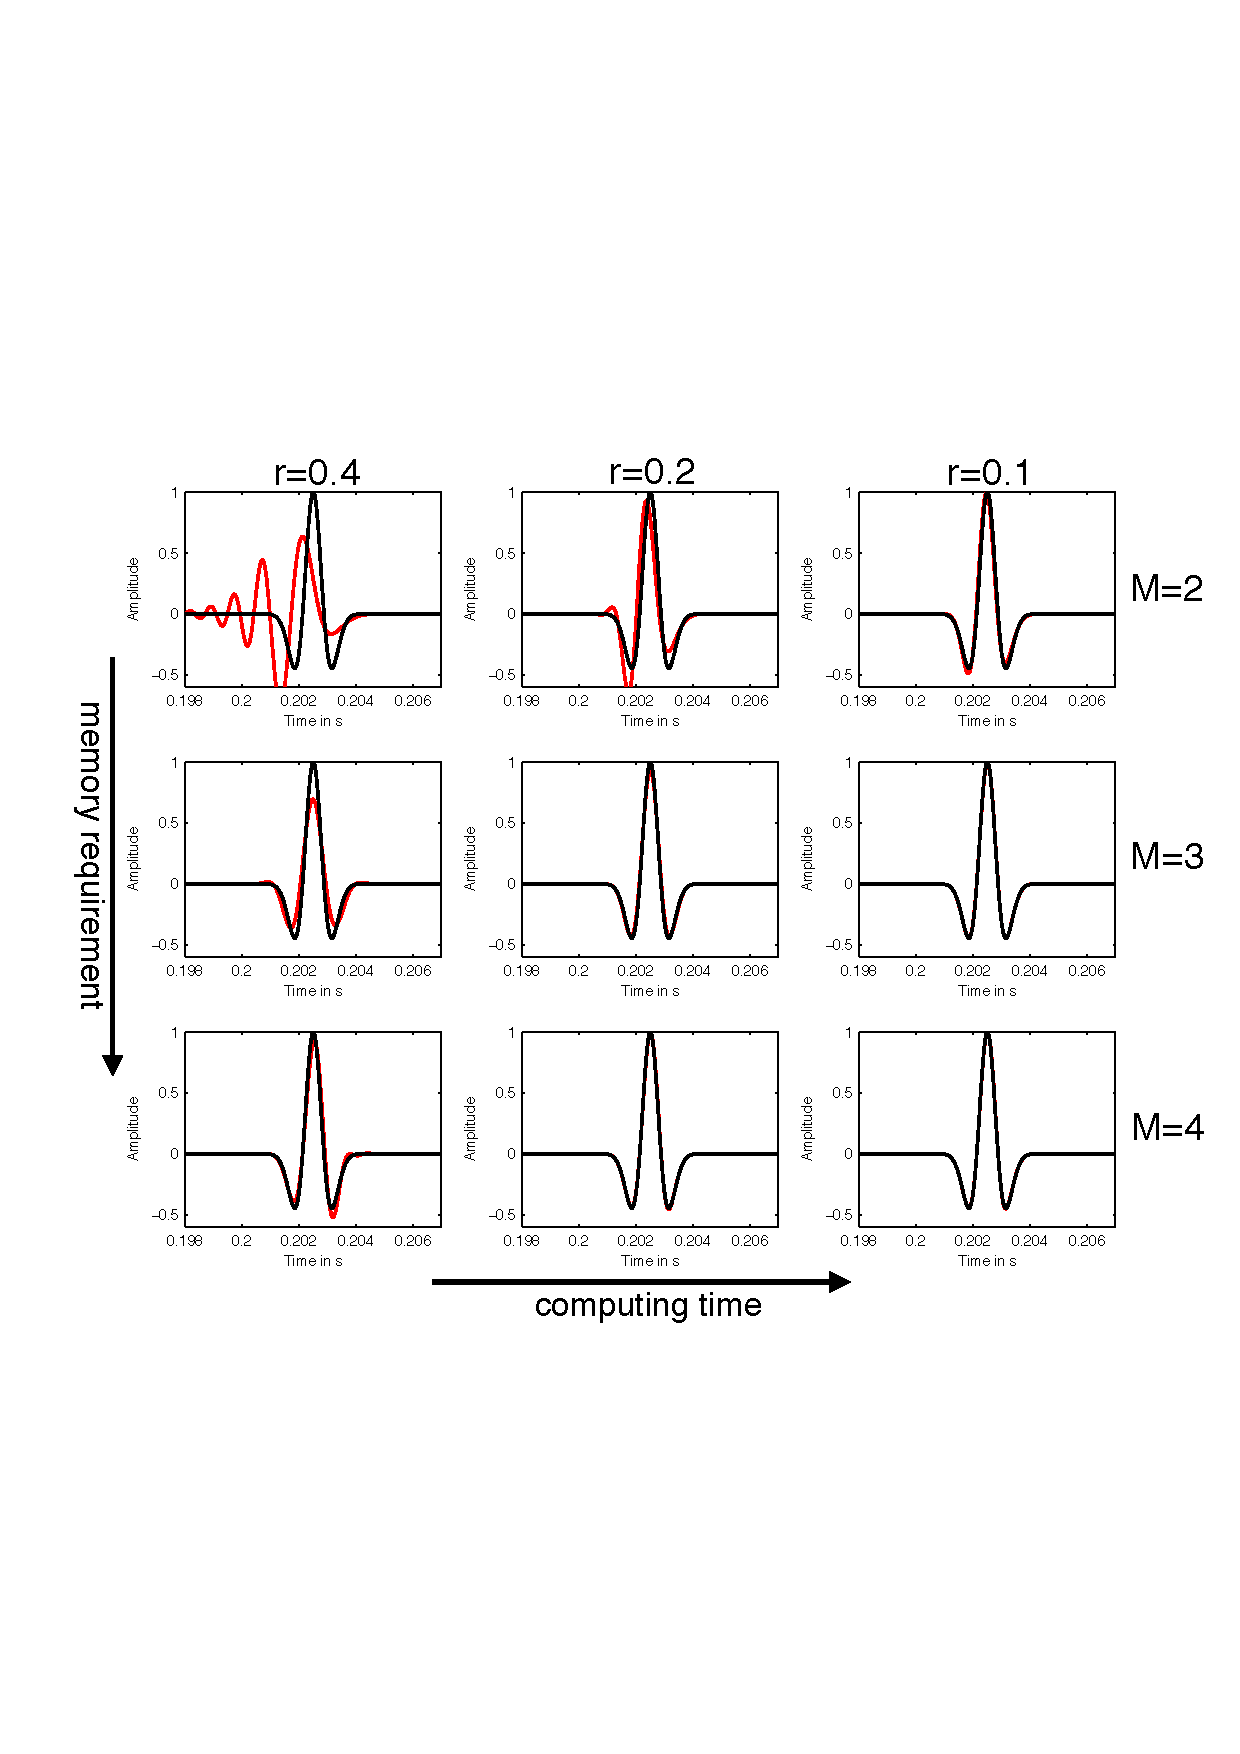
\includegraphics[width=\textwidth]{figures/seismo.pdf}
    \caption{Seismograms (red lines) calculated for the 1-D case for different Courant numbers $r$ and accuracy orders $M$. $M=2$ corresponds to the classical second order leapfrog scheme (Eq.~\ref{2ndorder}). $M=3,4$ correspond to the multi-step ABS method (Eq.~\ref{absmethod}). The analytical solution is plotted as a black line.}
    \label{fig_1dfdseis}
\end{figure}

\begin{figure}[h]
\centering
    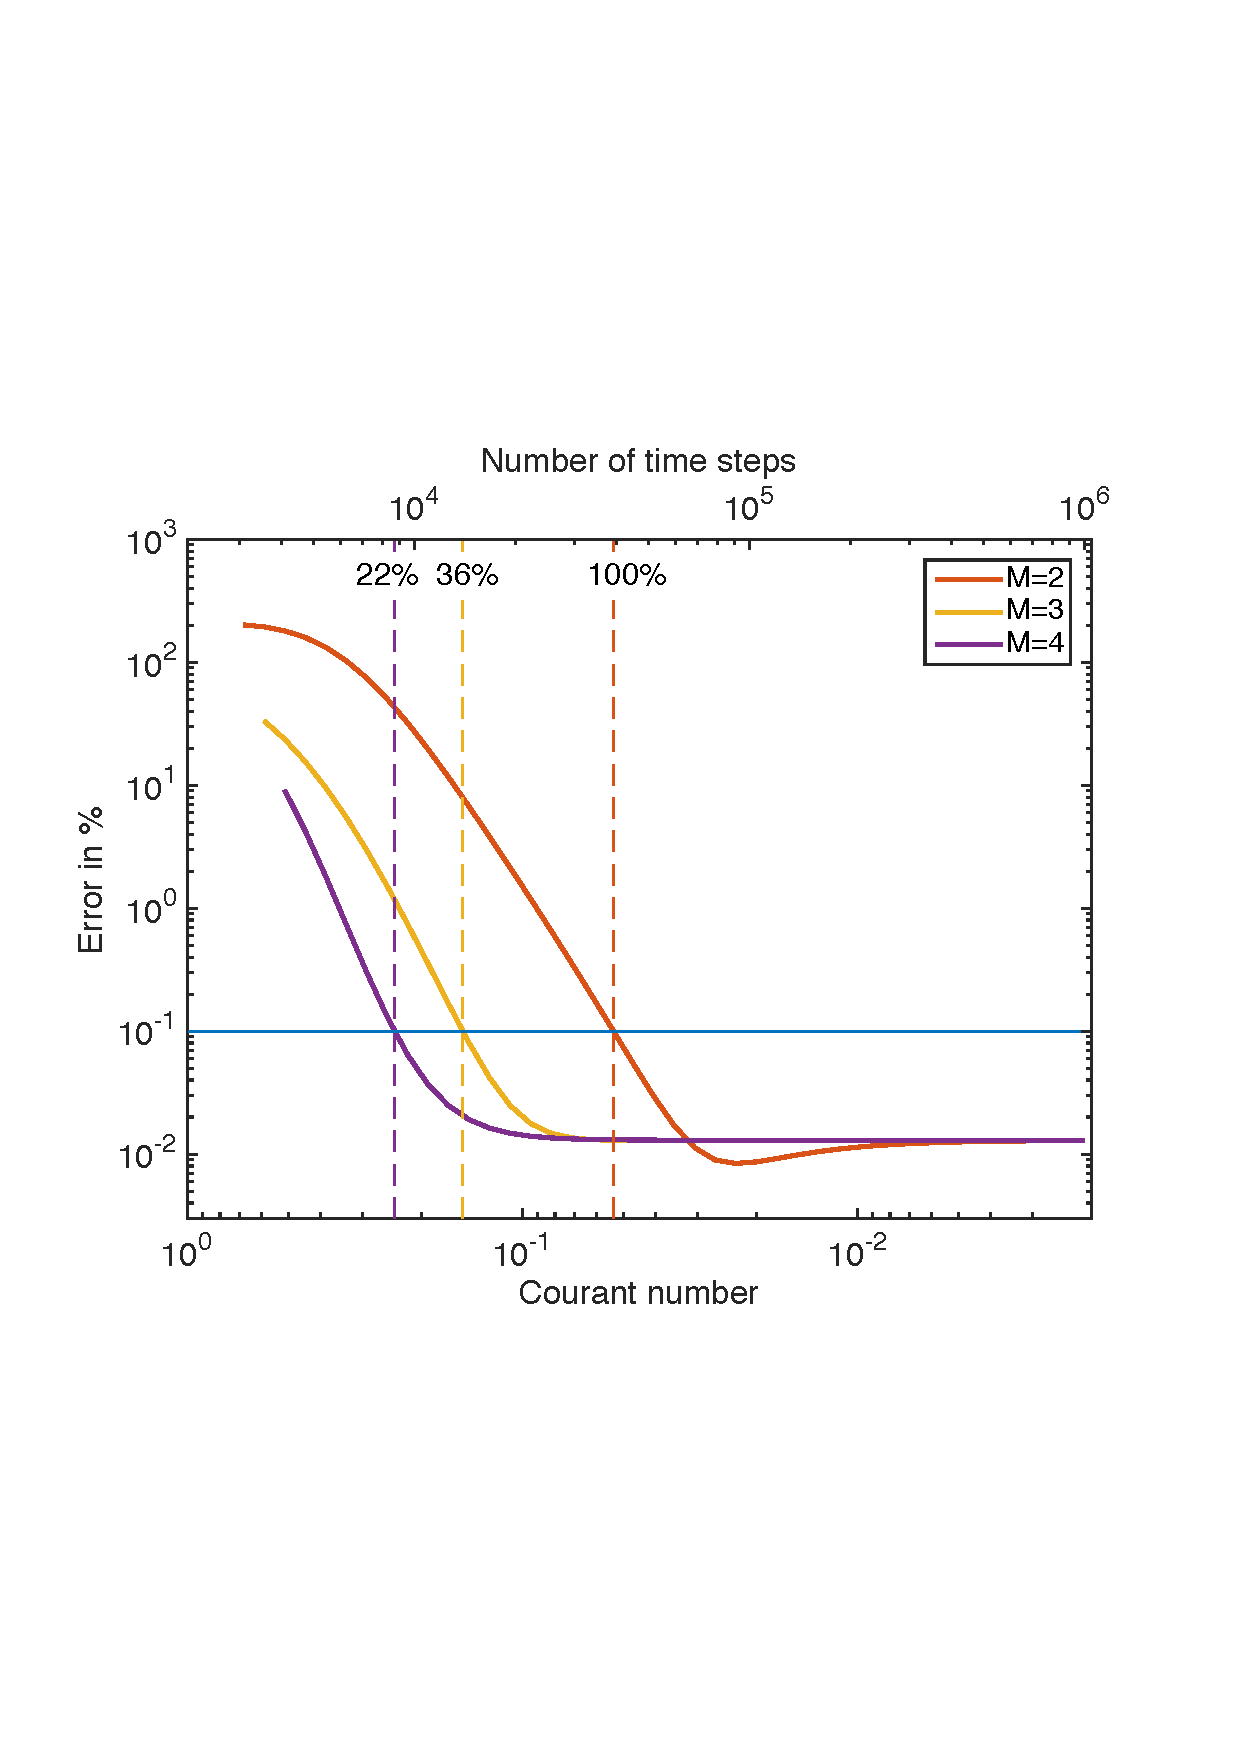
\includegraphics[scale=0.7]{figures/error_1D_courant}
    \caption{Relative error of 1D simulations (Fig.~\ref{fig_1dfdseis}). The normalized L2 norm is plotted over the required number of time steps ($NT$). The temporal accuracy orders are $M=2,3,4$. The spatial accuracy is fixed at order $N=8$. The number of time steps to achieve a given accuracy of $E=0.01\%$ (horizontal line) reduce to $36\%$ and $22\%$ for the temporal orders $M=3$ and $M=4$, respectively. For large $NT$ (small time step intervals) the error converges to the fixed error of the spatial discretization.}
    \label{fig_L2}
\end{figure}

\subsubsection{Absorbing Boundary Conditions}
Due to limited computational resources, the FD grid has to be as small as possible. To model problems with an infinite extension in different directions, e.g., a full or half-space problem,  an artificial absorbing boundary condition has to be applied. A very effective way to damp the waves near the boundaries are {\textbf{Perfectly Matched Layers (PMLs)}}. This can be achieved by a coordinate stretch of the wave equations in the frequency domain \cite{komatitsch:07}. The coordinate stretch creates exponentially decaying plane wave solutions in the absorbing boundary frame. The PMLs are only reflectionless if the exact wave equation is solved. As soon as the problem is discretized (for example using finite differences) you are solving an approximate wave equation and the analytical perfection of the PML is no longer valid. In SOFI2D, a damping profile $d_x$ after \citet{collino2001application} is implemented:
\begin{equation}
    d_x(x) = d_0\left(\frac{x}{L}\right)^n\;,
\end{equation}
where $L$ denotes the width of the absorbing frame and $d_0$ is a function of the theoretical reflection coefficient $R$:
\begin{equation}
    d_0 = -\left(n+1\right) V_{PML}\frac{log(R)}{2L}\;,
\end{equation}
where $V_{PML}$ denotes the typical P-wave velocity of the medium in the absorbing boundary frame. A reflection coefficient of $R=1 \times 10^{-4}$ is assumed. The PMLs are damping the seismic waves by a factor 5-10 more effective than the conventional absorbing boundary frame.

\subsection{Numerical artifacts and instabilities}
\label{num_instab}
To avoid numerical artifacts and instabilities during a FD modeling run, a spatial and temporal sampling condition for the wavefield has to be satisfied. These will be discussed in the following two sections. 

\subsubsection{Grid Dispersion}
\label{grid-dispersion}
The first question when building a FD model is: What is the maximum spatial grid point distance $\Delta h$, for a correct sampling of the wavefield? To answer this question we take a look at this simple example: The particle displacement in $x$-direction is defined by a sine function:
\begin{equation}
   v_x=\sin\biggl(2 \pi \frac{x}{\lambda}\biggr) \;,
   \label{eq:gri_disp}
\end{equation}
where $\lambda$ denotes the wavelength. When calculating the derivation of this function analytically at $x=0$ and setting $\lambda=\SI{1}{m}$ we get:
\begin{equation}
    \frac{d v_x}{d x}\biggl|_{x=0} = \frac{2 \pi}{\lambda} \cos\biggl(2 \pi \frac{x}{\lambda}\biggr)\biggl|_{x=0}=2 \pi\;.
    \label{eq:gri_disp_anal}
\end{equation}
In the next step the derivation is approximated numerically by a staggered 2nd order finite-difference operator:
\begin{equation}
    \frac{d v_x}{d x}\biggl|_{x=0} \approx \frac{v_x(x+\frac{1}{2}\Delta x)-v_x(x-\frac{1}{2}\Delta x)}{\Delta x}\biggl|_{x=0}=\frac{\sin \biggl(\frac{2 \pi (\frac{1}{2}{\Delta x})}{\lambda} \biggr)-\sin \biggl(\frac{2 \pi (\frac{1}{2}{dx})}{\lambda} \biggr)}{\Delta x}\;.
    \label{eq:gri_disp_num}
\end{equation}

Using the Nyquist-Shannon sampling theorem it should be sufficient to sample the wavefield with $\Delta x = \lambda/2$. In Table~\ref{grid_disp.1} the numerical solutions (Eq.~\ref{eq:gri_disp_num}) and the analytical solution (Eq.~\ref{eq:gri_disp_anal}) are compared for different sample intervals $\Delta x = \lambda /n$, where $n$ is the number of gridpoints per wavelength. For the case $n=2$, which corresponds to the Nyquist-Shannon theorem, the numerical solution is $\frac{d v_x}{d x}|_{x=0}=4.0$, which is not equal with the analytical solution $2 \pi$. A refinement of the spatial sampling of the wavefield results in an improvement of the finite difference solution. For $n=16$ the numerical solution is accurate to the second decimal place. The effect of a sparsely sampled pressure field is illustrated in Fig.~\ref{fig_homo_grid} for a homogeneous block model with stress free surfaces. The dimensions of the FD grid are fixed and the central frequency of the source signal is increased systematically.  When using a spatial sampling of 16 grid points per minimum wavelength (\ref{fig_homo_grid}, top) the wavefronts are sharply defined. For $n=4$  grid points a slight numerical dispersion of the wave occurs (\ref{fig_homo_grid}, center). This effect is obvious when using the Nyquist criterion ($n=2$) (\ref{fig_homo_grid}, bottom). Since the numerical calculated wavefield seem to be dispersive this numerical artefact is called {\textbf{grid dispersion}}. 

To avoid the occurence of grid dispersion the following criteria for the spatial grid spacing $\Delta h$ has to be satisfied:
\begin{equation}
    \Delta h \le \frac{\lambda_{min}}{n} = \frac{V_{min}}{{n}\,f_{max}}\;,
    \label{eq:dh}
\end{equation}
where $\lambda_{min}$ denotes the minimum wavelength, $V_{min}$ the minimum velocity in the model, and $f_{max}$ is the maximum frequency of the source signal.  

Depending on the accuracy of the used FD operator the parameter $n$ is different. In Table~\ref{grid_disp.2} n is listed for different FD operator lengths and types (Taylor and Holberg operators). The Holberg coefficients are calculated for a minimum dispersion error of $0.1\%$ at $3 f_{max}$. For short operators n should be chosen relatively large, so the spatial grid spacing is small, while for longer FD operators n is smaller and the grid spacing can be larger. 
\begin{figure}[ht!]
\centering
    \begin{subfigure}[b]{0.45\textwidth}
        \centering
        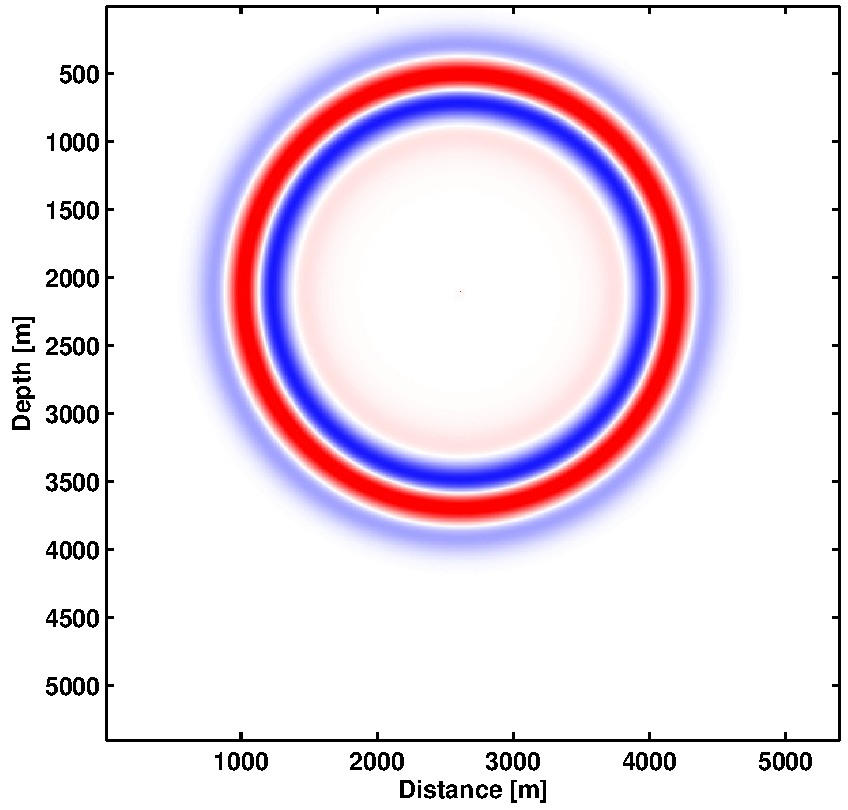
\includegraphics[width=\textwidth]{figures/homogenous_grid_n_16_5.pdf}
        \caption{}
    \end{subfigure}
    \hfill
    \begin{subfigure}[b]{0.45\textwidth}
        \centering
        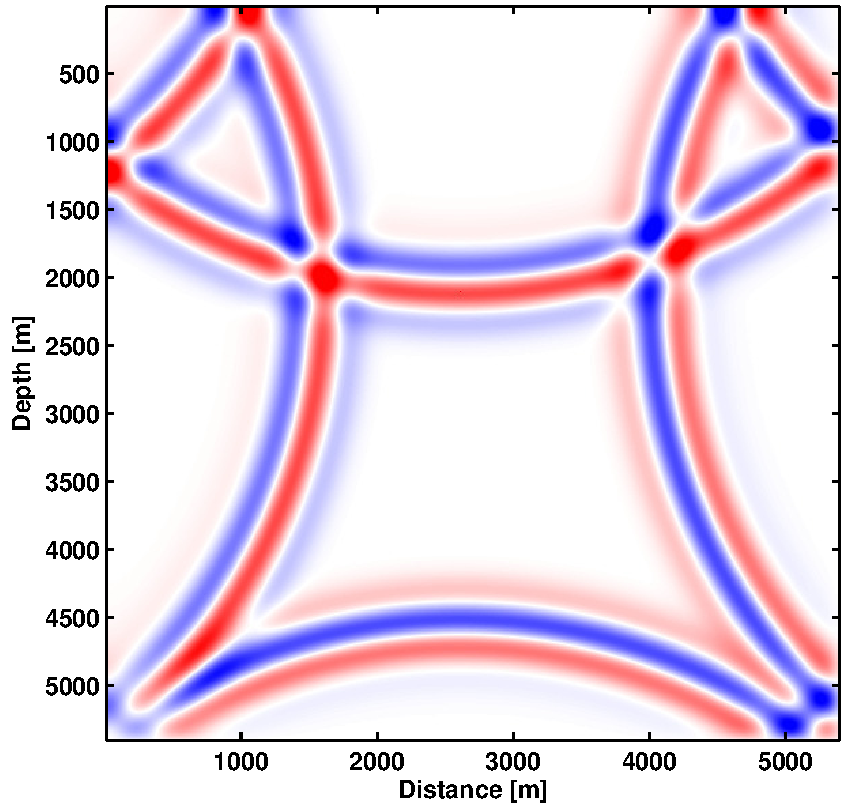
\includegraphics[width=\textwidth]{figures/homogenous_grid_n_16_10.pdf}
        \caption{}
    \end{subfigure}
    \vfill
    \begin{subfigure}[b]{0.45\textwidth}
        \centering
        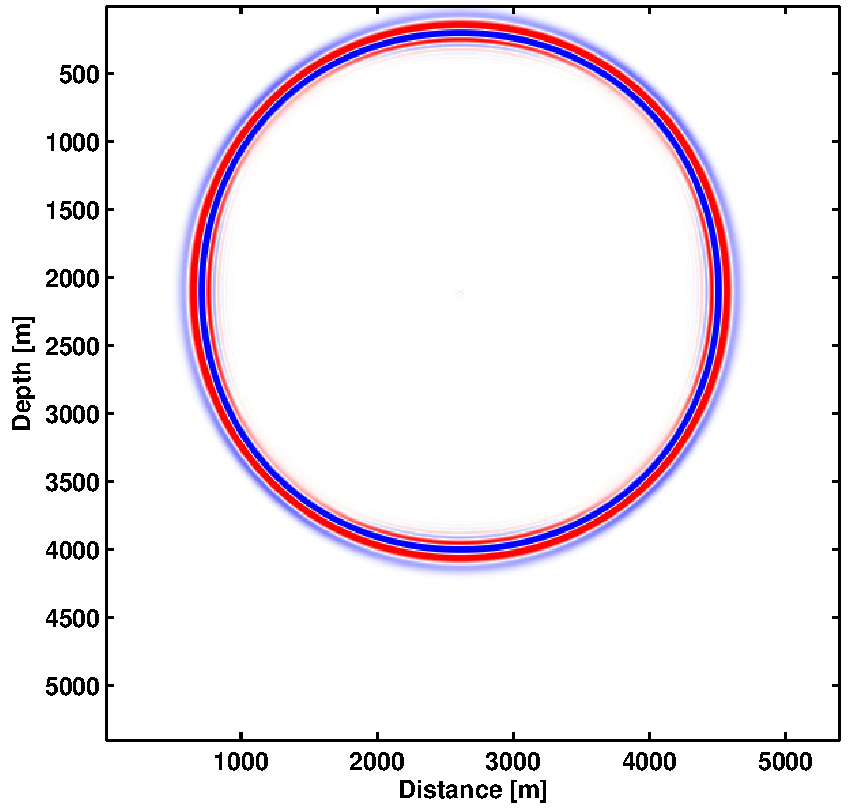
\includegraphics[width=\textwidth]{figures/homogenous_grid_n_4_5.pdf}
        \caption{}
    \end{subfigure}
    \hfill
    \begin{subfigure}[b]{0.45\textwidth}
        \centering
        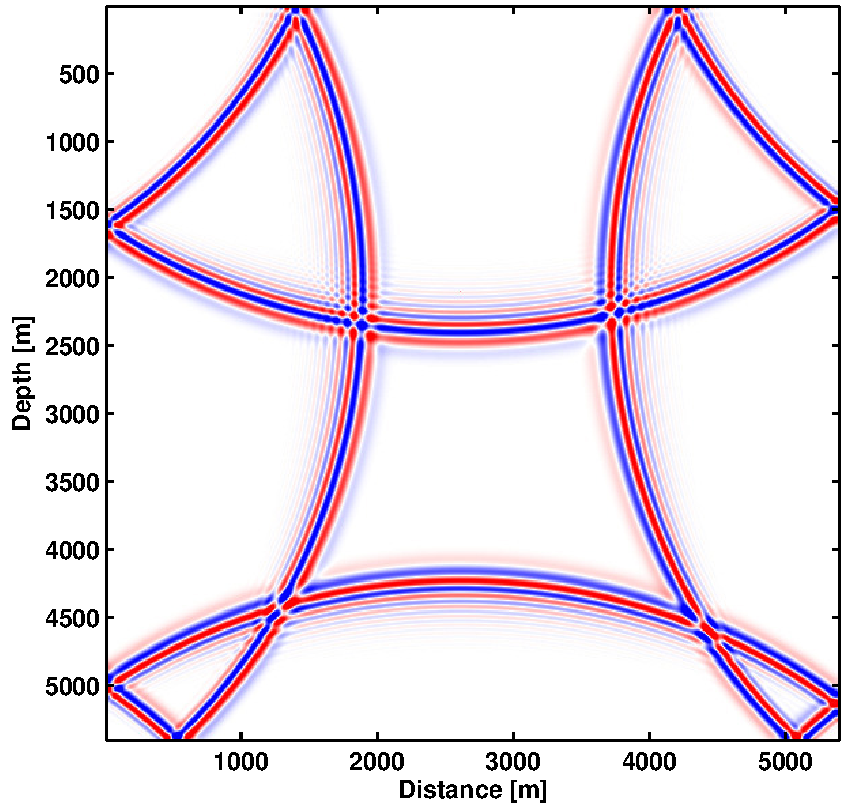
\includegraphics[width=\textwidth]{figures/homogenous_grid_n_4_10.pdf}
        \caption{}
    \end{subfigure}
    \vfill
    \begin{subfigure}[b]{0.45\textwidth}
        \centering
        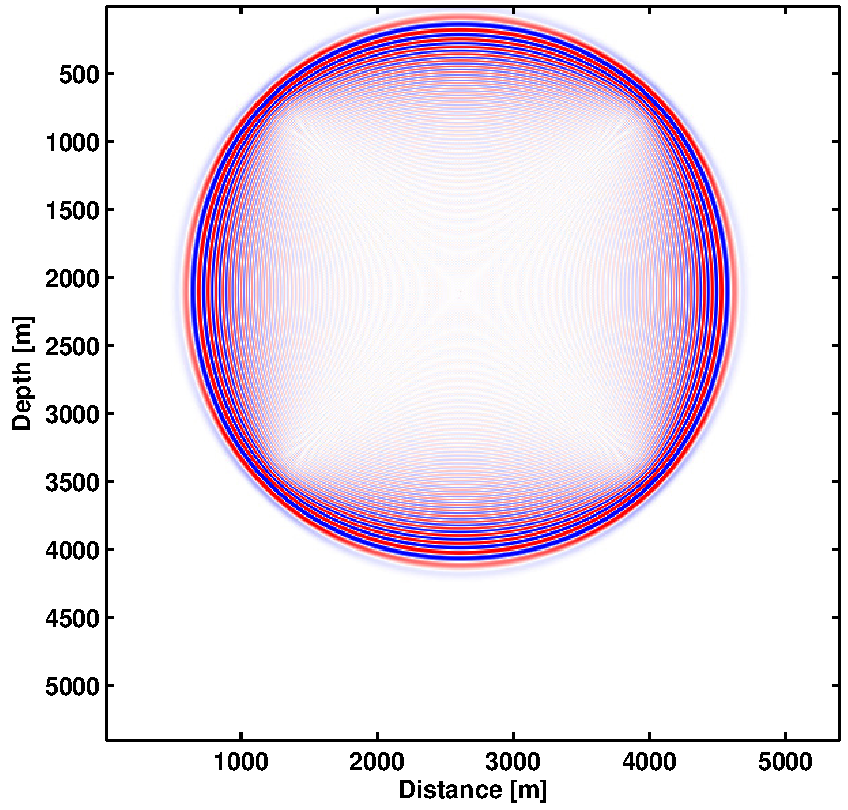
\includegraphics[width=\textwidth]{figures/homogenous_grid_n_2_5.pdf}
        \caption{}
    \end{subfigure}
    \hfill
    \begin{subfigure}[b]{0.45\textwidth}
        \centering
        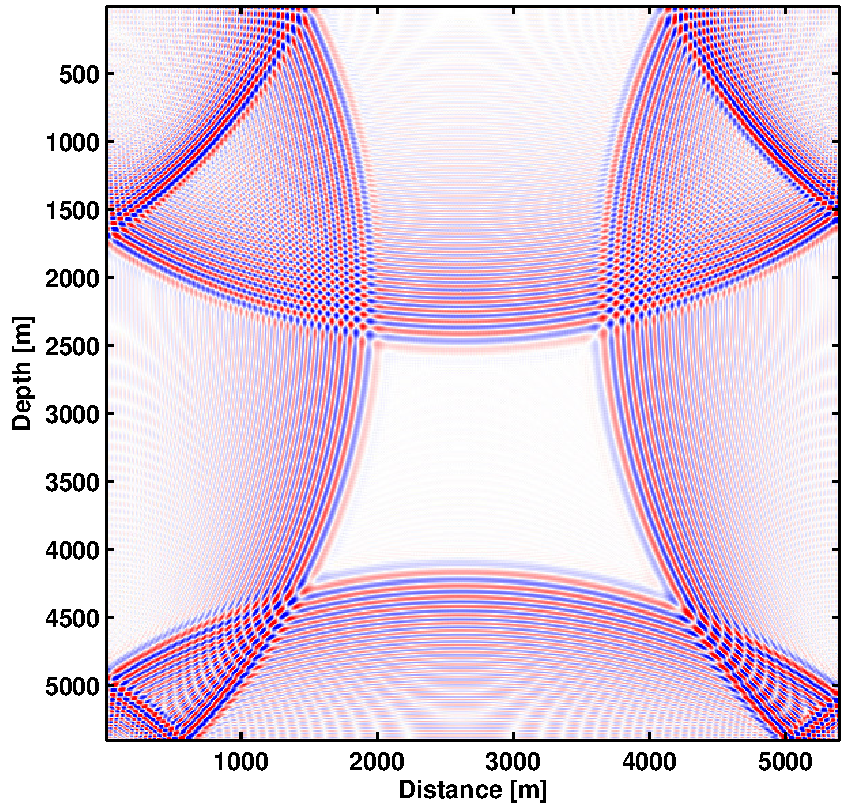
\includegraphics[width=\textwidth]{figures/homogenous_grid_n_2_10.pdf}
        \caption{}
    \end{subfigure}
\caption{\label{grid_disp_pics} The influence of grid dispersion in FD modeling: Spatial sampling of the wavefield using $n=16$ (top), $n=4$ (center) and $n=2$ gridpoints (bottom) per minimum wavelength.}
\label{fig_homo_grid}
\end{figure}

\begin{table}[hbt]
\caption{\label{grid_disp.1} Comparison of the analytical solution Eq.~\ref{eq:gri_disp_anal} with the numerical solution Eq.~\ref{eq:gri_disp_num} for different grid spacing $\Delta x = \lambda /n$.}
\centering
\begin{tabular}{c|c|c}
    \textbf{n} &  \textbf{$\mathbf{\Delta x}\,$ [m]} & \textbf{$\mathbf{\frac{d v_x}{d x}|_{x=0}}$} \\ \hline 
    analytical & - & $2\pi \approx 6.283$ \\ 
    2 & $\lambda/2$ & 4.0 \\ 
    4 & $\lambda/4$ & 5.657 \\ 
    8 & $\lambda/8$ & 6.123 \\ 
    16 & $\lambda/16$ & 6.2429 \\ 
    32 & $\lambda/32$ & 6.2731
\end{tabular}
\end{table}
 
\begin{table}[hbt]
\caption{\label{grid_disp.2} The number of grid points per minimum wavelength $n$ for different orders (2nd-12th) and types (Taylor and Holberg) of FD operators. For the Holberg coefficients n is calculated for a minimum dispersion error of $0.1\%$ at $3\,f_{max}$.}
\centering
\begin{tabular}{c|c|c}
    \textbf{FDORDER} & \textbf{n (Taylor)} & \textbf{n (Holberg)} \\ \hline 
    2nd   &   12       &  12         \\
    4th   &   8        &  8.32       \\
    6th   &   6        &  4.77       \\
    8th   &   5        &  3.69       \\ 
    10th  &   5        &  3.19       \\
    12th  &   4        &  2.91       
\end{tabular}
\end{table} 

\subsubsection{The Courant Instability}
\label{courant}
Beside the spatial, the temporal discretization has to satisfy a sampling criterion to ensure the stability of the FD code. If a 
wave is propagating on a discrete grid, then the timestep $\Delta t$ has to be less than the time for the wave to travel between two adjacent grid 
points with grid spacing $\Delta h$. For an elastic 2D grid this means mathematically:
\begin{equation}
    \Delta t \le \frac{\Delta h}{h \sqrt{2} V_{max}}\;,
    \label{courant_crit}
\end{equation}
where $V_{max}$ is the maximum velocity in the model. The factor $h$ depends on the order of the FD operator and can easily calculated by summing over the weighting coefficients $\beta_i$: $h = \sum_i \beta_i$. In Table~\ref{courant.1} $h$ is listed for different FD operator lengths and types (Taylor and Holberg operators). Criterion Eq.~\ref{courant_crit} is called {\textbf{Courant-Friedrichs-Lewy criterion}} (\cite{courant:28}, \cite{courant:67}). 
Fig.~\ref{fig_courant} shows the evolution of the pressure field when the Courant criterion is violated. After a few time steps the amplitudes are growing to infinity and the calculation becomes unstable.
\begin{figure}[ht!]
\centering
    \begin{subfigure}[b]{0.45\textwidth}
        \centering
        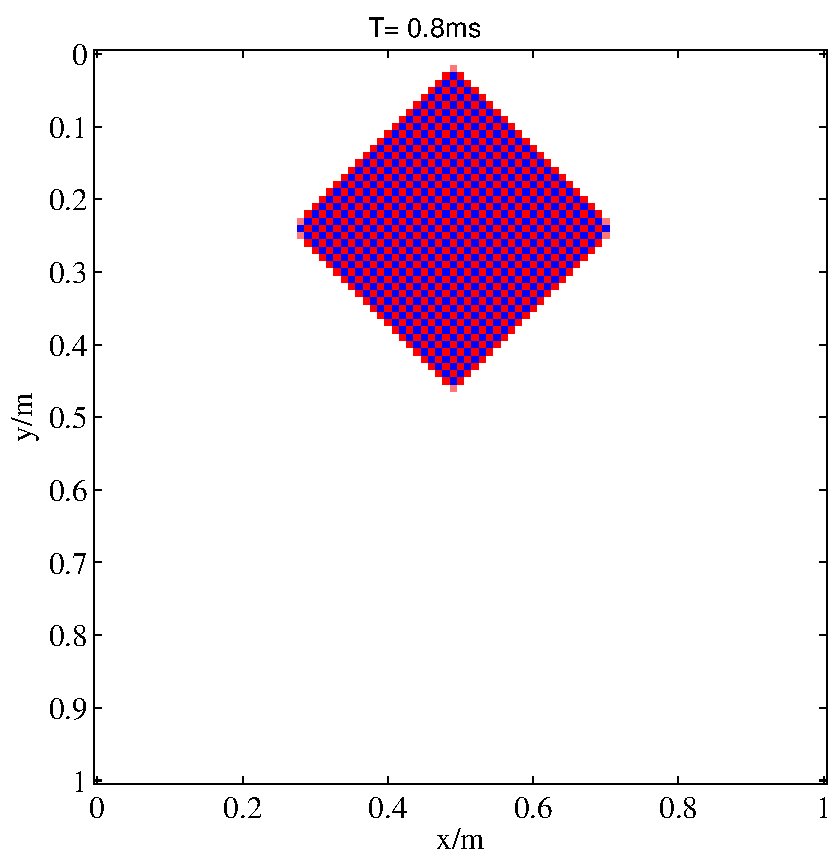
\includegraphics[width=\textwidth]{figures/courandt_1.pdf}
        \caption{}
    \end{subfigure}
    \hfill
    \begin{subfigure}[b]{0.45\textwidth}
        \centering
        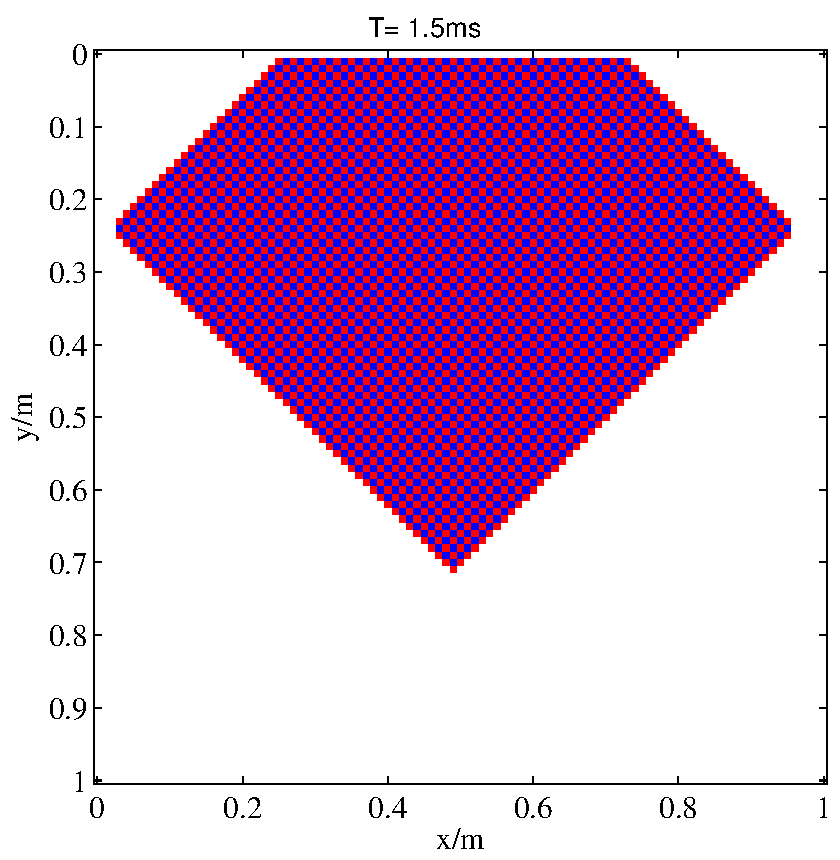
\includegraphics[width=\textwidth]{figures/courandt_2.pdf}
        \caption{}
    \end{subfigure}
    \vfill
    \begin{subfigure}[b]{0.45\textwidth}
        \centering
        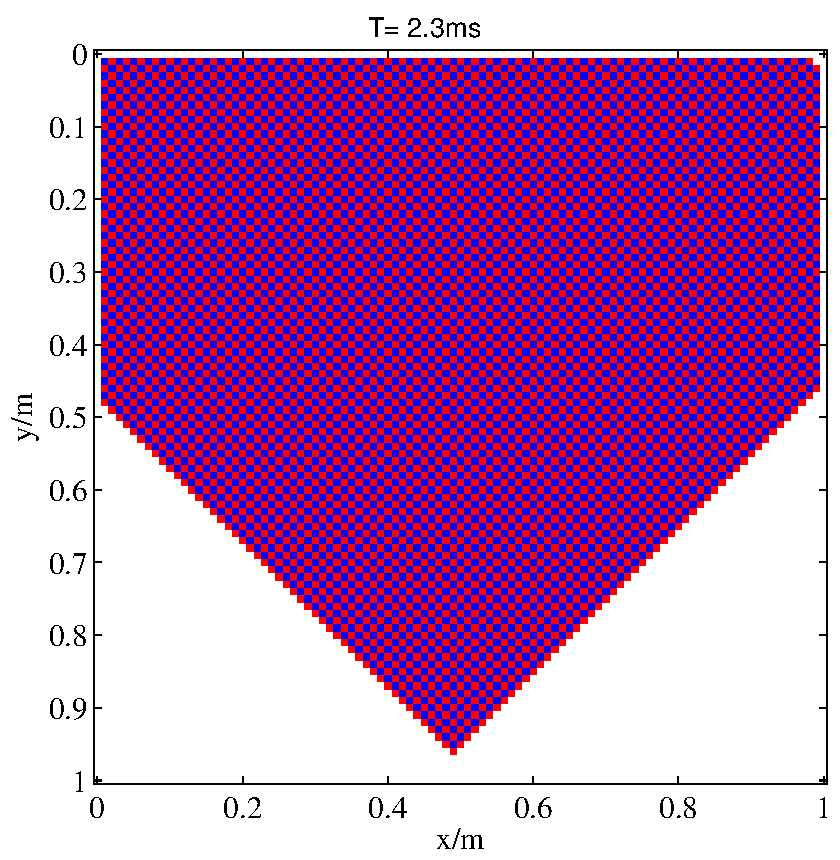
\includegraphics[width=\textwidth]{figures/courandt_3.pdf}
        \caption{}
    \end{subfigure}
    \hfill
    \begin{subfigure}[b]{0.45\textwidth}
        \centering
        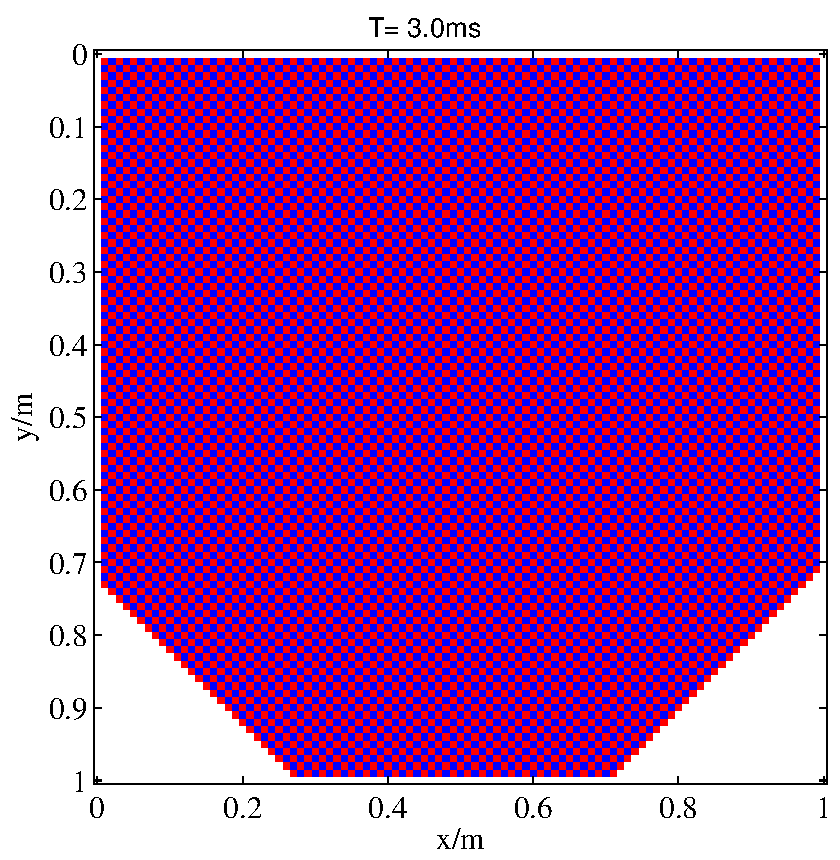
\includegraphics[width=\textwidth]{figures/courandt_4.pdf}
        \caption{}
    \end{subfigure}
    \caption{\label{courant_pics} Temporal evolution of the Courant instability. In the colored areas the wave amplitudes are extremely large.}
\label{fig_courant}
\end{figure}

\begin{table}[hbt]
\caption{\label{courant.1} The factor $h$ in the Courant criterion for different orders (2nd-12th) and types (Taylor and Holberg) of FD operators.}
\centering
\begin{tabular}{c|c|c}
\textbf{FDORDER} & \textbf{h (Taylor)}      & \textbf{h (Holberg)} \\ \hline
2nd   &   1.0             &  1.0        \\
4th   &   7/6             &  1.184614   \\
6th   &   149/120         &  1.283482   \\
8th   &   2161/1680       &  1.345927   \\
10th  &   53089/40320     &  1.387660   \\
12th  &   1187803/887040  &  1.417065    
\end{tabular}
\end{table} 
